\section{Notions of complex dynamics}\label{complexdynamics}
\subsection{Generalities on the subject}
Here we summarize the necessary notions on dynamics of rational functions in the complex plane needed for our work. Sources like \cite{beardon} and \cite{milnordynamics} are recommended for the interested reader for more detailed information in complex dynamics. All prerequisites from complex analysis are covered in \cite{ahlfors}. If $f:X \rightarrow X$ is a function, we shall denote by $f^n$ the composition of $f$ with itself $n\geq 1$ times, and by definition $f^0$ is the identity map on $X$.

\begin{mydef}{}{def01}
A family of functions $\{g_i\}_{i\in I}$ acting on a metric space $(X,d)$ is said to be {\bf equicontinuous} at $x \in X$ if for any $\varepsilon>0$ there exists $\delta>0$ such that $d(x,y)<\delta$ implies $d(g_i(x),g_i(y))<\varepsilon$ for all $i \in I$. If the family is equicontinuous at every point of some subset $A\subset X$, then we will say that the family is equicontinuous on $A$.
\end{mydef}

Consider the metric space $(\C,\sigma)$ where $\C$ is the Riemann sphere \nomenclature[01]{$\C$}{The Riemann sphere} and $\sigma$ is the spherical metric, that is, $\sigma(z,w)$ is the Euclidean length of the shortest path between $z$ and $w$ viewed as points in $S^2=\{x\in \mathbb{R}^3\,:\, \|x\|=1\}$. Take a non-constant rational map $f:\widehat{\mathbb{C}} \rightarrow \widehat{\mathbb{C}}$, and suppose that the family $\{f^{n}\}_{n\geq 1}$ of forward iterations of $f$ results to be equicontinuous on a set $A$. Then, for any $z\in A$ there is $\delta = \delta(z,\varepsilon)$ such that $\sigma(z,w)<\delta$ implies $\sigma(f^n(z),f^n(w))<\varepsilon$ for all $n\geq 1$. In such case $f$ presents some sort of stability on $A$, in the sense that orbits of $f$ which have sufficiently close initial conditions will remain close at every iteration by $f$, so the orbits are not sensitive to initial conditions.\\

Now, since equicontinuity is a definition given pointwise, if $\{g_i\}_{i\in I}$ is equicontinuous on $A$ and $B$ then it is equicontinuous on $A\cup B$. More generally, if a family of funtions is equicontinuous on $\{A_j\}_{j\in J}$ then it is equicontinuous on $\bigcup_{j\in J} A_j$. These observations lead to the following definition.

\begin{mydef}{}{JuliaF}
The {\bf Fatou set} of a rational map $f$ of degree $d\geq 1$ is defined to be the maximal open set in $\C$ on which the family $\{f^n\}_{n\geq 1}$ is equicontinuous. It is denoted as $F(f)$. \nomenclature[02]{$F(f)$}{Fatou set of $f$} The {\bf Julia set} associated to $f$ is defined as $J(f) \coloneqq \C\setminus F(f)$. \nomenclature[03]{$J(f)$}{Julia set of $f$}
\end{mydef}

By definition, $F(f)$ is an open subset whereas $J(f)$ is a compact subset of $\C$. Notice that in principle there is no reason to suppose that $J(f)$, or $F(f)$, is non-empty for a given rational  function $f$. In fact, the identity function $f(z)=z$ is an example for which $J(f)=\emptyset$. On the other hand, $f(z) = (z^2+1)^2/(4z(z^2-1))$ is an example of a function with $J(f) = \C$, see \cite[Section 4.3]{beardon}. However, we can prove that if $f$ has degree at least $2$ then $J(f)\neq \emptyset$. For this, we need to recall the notion of normality.

\begin{mydef}{}{defnormality}
Let $X,Y$ be metric spaces. A family of functions $\{g_i:X\to Y \}_{i\in I}$ is said to be {\bf normal} on $A\subset X$ if every sequence of the family contains a subsequence which converges uniformly on compact subsets of $A$.
\end{mydef}

The version of Arzela-Ascoli's Theorem in \cite[Theorem 14, Section 5.3]{ahlfors} implies that the family of iterations of a rational map $\{f^n\}_{n\geq 1}$ is normal on an open subset $\Omega\subset \C$ if and only if it is equicontinuous on every compact subset $K\subset \Omega$. Particularly, $\{f^n\}_{n\geq 1}$ is a normal family precisely on $F(f)$. Now we can prove the following proposition.

\begin{myprop}{}{propjulianonempty}
If $f:\C \rightarrow \C$ is a rational function of degree at least $2$ then $J(f) \neq \emptyset$.
\end{myprop}

\begin{proof}
Suppose on the contrary that $J(f)=\emptyset$, then there is a sequence of integers $\{n_k\}_{k\geq 1}$ such that $f^{n_k}$ converges uniformly on $\C$ to a meromorphic function. The limit must be then a rational map. Hence, the degrees of each $f^{n_k}$ must stabilize for large enough $n_k$. This is only possible if $f$ is a rational map of degree $1$, which is a contradiction. Therefore $J(f)\neq \emptyset$.
\end{proof} 

\begin{myexmp}{}{zalan}
Let $f(z) = z^m$ for some $|m|\geq 2$. Then it is readily seen that $f^n(z)\rightarrow 0$ uniformly on compact subsets of $\D\coloneqq \{|z|<1\}$ \nomenclature[04]{$\mathbb{D}$}{The unitary disk in $\mathbb{C}$} as $n\rightarrow \infty$. Similarly, considering $f$ as a function on $\widehat{\mathbb{C}}$ it happens that $f^n(z)\rightarrow \infty$ uniformly on compact subsets of $\{|z|>1\}\subset \C$ as $n\rightarrow \infty$. Hence $\D\cup \{|z|>1\} \subset F(f)$. On the other hand, in every neighborhood of a point $w\in \partial \D$ there are points which converge to $0$ under iteration by $f$, and points which converge to $\infty$. Hence $\{f^n\}_{n\geq 1}$ cannot be equicontinuous on any neighborhood of any point in $\partial \D$. We conclude that $J(f)=\partial D$ and thereby $F(f)$ is its complement in $\C$.   
\end{myexmp}

\begin{myexmp}{}{ejemploblashky}
It is known that every automorphism of the unitary disk $\D$ is of the form $\phi_a(z) = e^{i\theta}(z-a)/(1-\overline{a}z)$ for some $\theta\in \mathbb{R}$ and some $a\in \D$ \cite[Chapter 8, Theorem 2.2]{stein}. Since Möbius transformations are determined by their action in three distinct points, it is easily deduced that each $\phi_a$ maps $\partial \D$ onto itself. It can be deduced then that an expression of the form
\begin{equation}\label{defblashky}
f(z) = e^{i\theta} \phi_{a_1}(z)\phi_{a_2}(z)\cdots \phi_{a_n}(z), \qquad a_j\in \D,
\end{equation}
preserves $\partial \D$ and carries $\D$ onto $\D$ and $\C \setminus \overline{\D}$ onto $\C \setminus \overline{\D}$. Every function as in Equation \eqref{defblashky} is called a {\bf Blaschke product}. Hence, if $f$ is a Blaschke product, by applying Montel's Theorem it can be deduced that the family of iterations of $f$ is normal on $\D$ and on $\C \setminus \overline{\D}$, see Theorem \ref{th:Montel}. Hence $J(f)\subset \partial \D$. Now, suppose that some factor in \eqref{defblashky} is $\phi_0(z)=z^2$, then $f^n(z) \rightarrow 0$ if $|z|<1$ and $f^n(z) \rightarrow \infty$ if $|z|>1$. So in this case we can assure that $J(f) = \partial \D$. Similar statements hold for any function $f(z)=z^n\frac{z-a}{1-\overline{a}z}$ with $0<|a|<1$ and $n\geq 2$.
\end{myexmp}

We proceed to develop some properties of the Julia and Fatou sets that we will need later.\\

\begin{myprop}{}{conjugation}
If $f$ is a non-constant rational map and $g$ is a Möbius transformation let $S= g\circ f\circ g^{-1}$, then $F(S) = g(F(f))$ and $J(S)=g(J(f))$. 
\end{myprop}

\begin{proof}
Since every Möbius transformation is a homeomorphism of $\C$, we have that $f^{n_k}$ converges uniformly on a compact set $K$ if and only if $S^{n_k}=g\circ f^{n_k} \circ g^{-1}$ converges uniformly on $g(K)$. Hence, $S$ is normal precisely in $g(F(f))$ and the result follows.
\end{proof}

Now we study invariance properties of the Fatou and Julia sets under iteration of the rational map they are associated with. Let us give precise definitions of the different kinds of invariance we are interested in.\\
 
\begin{mydef}{}{definvariance}
Let $f$ be a function on a metric space $X$. We say that a subset $A\subset X$ is {\bf forward invarant} under $f$ if $f(A)\subset A$, {\bf backward invariant} if $f^{-1}(A)\subset A$, and {\bf completely invarant} if $A$ is forward invariant and backward invariant under $f$.
\end{mydef}

To prove the next proposition we need to recall a topological concept. An {\bf exhaustion} of an open set $\Omega$ is a sequence of compact subsets $\{K_i\}_{i=1}^n$, each contained in $\Omega$, such that $K_i \subset \text{int}(K_{i+1})$ for every $i\geq 1$ and $\Omega = \cup_{i\geq 1} K_i$.

\begin{mylema}{}{lemaexaustion}
Every open set $\Omega\subset \C$ has an exhaustion.
\end{mylema}
 
\begin{proof}
For each $i\geq 1$, define $K_i$ as the set of points in $\Omega$ which are at distance at least $1/i$. Here we are considering the spherical metric on $\C$. Then the sequence $\{K_i\}_{i\geq 1}$ is an exhaustion for $\Omega$.
\end{proof}

\begin{myprop}{}{completely invariance}
Let $f$ be a non-constant rational function over $\C$. Then $F(f)$ and $J(f)$ are completely invariant under $f$. Moreover, for any $p\geq 1$ we have that $F(f^p)=F(f)$ and $J(f^p) = J(f)$.
\end{myprop}

\begin{proof}
Let $K\subset \C$ be a compact set and suppose that $\{f^n\}_{n\geq 1}$ is normal on $K$, then so is in $f(K)$ since if $f^{n_k}$ converges at $z\in K$ so does $f^{n_k-1}$ at $f(z)\in f(K)$, therefore $f(F(f))\subset F(f)$. Similarly, if $\{f^n\}$ is equicontinuous on $K$, by uniform continuity of $f$ on $f^{-1}(K)$ the family $\{ f^{n}\circ f\}_{n\geq 1} = \{f^{n}\}_{n\geq 2}$ is equicontinuous on $f^{-1}(K)$. Again, uniform continuity of $f$ on $f^{-1}(K)$ implies that $\{f^n\}_{n\geq 1}$ is equicontinuous in $f^{-1}(K)$. Now, by Lemma \ref{lm:lemaexaustion} $F(f)$ has an exhaustion by compact sets. We can deduce then that $f^{-1}(F(f))\subset F(f)$. The complete invariance follows.\\

Similarly, if $\{f^n\}_{n\geq 1}$ is equicontinuous on an open set so is the subfamily $\{f^{np}\}_{n\geq 1}$, and when $\{f^{np}\}$ is normal so is $\{f^n\}_{n\geq 1}$, hence $F(f^p)=F(f)$ from which it follows that $J(f^p)=J(f)$. 
\end{proof}

The continuity of a rational map and Proposition \ref{pr:completely invariance} imply that a connected component of $F(f)$ is mapped into some, but not necessarily different, connected component of $F(f)$. However, properties of holomorphic functions allow us to tell a bit more, which may not be necessarily true for dynamics in general metric spaces.\\

\begin{myprop}{}{componentfatouonto}
Let $f$ be a non-constant rational map over $\C$. Then each connected component of $F(f)$ is mapped under $f$ onto some other connected component of $F(f)$. 
\end{myprop}
\begin{proof}
Let $U\subset F(f)$ be a Fatou component and suppose it is mapped into some component $V\subset F(f)$ under $f$. The Open Mapping Theorem implies that $f(U)$ is open. Since $f(\overline{U})$ is closed, we deduce $f(\partial U) = \partial f(U)$. Now, $U$ is contained strictly in $V$ if and only if $V\cap \partial f(U) \neq \emptyset$. But $\partial U\subset J(f)$ so forward invariance of $J(f)$ implies that $\partial f(U)=f(\partial U)\subset J(f)$. Since $V\cap J(f)\subset F(f)\cap J(f)=\emptyset$ we get that necessarily $f(U)=V$.
\end{proof}

For later use, let us study now the possible finite sets which are completely invariant under a rational function, this will give rise to very important type of points kown as \emph{exceptional points}. First we introduce the concept of \emph{valency}. Let $f$ be a holomorphic function near $z_0\in \mathbb{C}$, then from its Taylor series expansion at $z_0$ it follows that there exists a unique integer $k\geq 1$ such that the limit
$$\lim_{z\rightarrow z_0} \frac{f(z)-f(z_0)}{(z-z_0)^k},$$
is finite and non-zero. The interger $k$ is called the {\bf valency} of $f$ at $z_0$ and will be denoted by $v_f(z_0)$ \nomenclature[05]{$v_f(z_0)$}{Valency of $f$ at $z_0$}. The point $z_0$ is a {\bf critical point} of $f$ if and only if $v_f(z_0)>1$ if and only if $f$ is not injective in any neighborhood of $z_0$. By definition $v_f(w)$ is the multiplicity of $w$ as a root of the equation $f(z)=f(w)$. Also, the multiplicity of a critical point $z_0$ of $f$ is $v_f(z_0)-1$, since it refers to the multiplicity of $z_0$ as a root of the equation $f'(z_0)=0$.\\

Now let $g$ be another holomorphic function such that $g\circ f$ is holomorphic near $z_0$. Let $q=v_g(f(z_0))$. As consequence of the following identity
$$\frac{g(f(z))-f(g(z_0))}{(z-z_0)^{kq}} = \frac{g(f(z))-g(f(z_0))}{(f(z)-f(z_0))^q} \cdot \left( \frac{f(z)-f(z_0)}{(z-z_0)^k}\right)^q,$$
the valency of $g\circ f$ at $z_0$ is $kq$, that is
\begin{equation}\label{chainrule}
v_{g\circ f}(z_0) = v_g(f(z_0))\cdot v_f(z_0).
\end{equation}
Particularly, composition with Möbius transformations does not alter the valency.\\

We can define also the valency of a meromorphic function at a pole. Suppose that $f$ has a pole at $z_0\in \C$, take Möbius transformations $g,h$ such that $g(z_0),h(\infty)\in \mathbb{C}$, define $F=h\circ f\circ g^{-1}$ and let
$$v_f(z_0) \coloneqq v_F(g(z_0)).$$
Notice that $F$ is holomorphic near $z_0$ so the righthand side in the previous equation makes sense. Nonetheless, we need show that the definition does not depend on the election of $g$ and $h$. An easy argument settles this issue: for any other Möbius transformations $\tilde{g},\tilde{h}$ satisfying $\tilde g(z_0),\tilde h(\infty)\in \mathbb{C}$, Equation \eqref{chainrule} implies that if $G=\tilde{h}\circ f \circ \tilde{g}^{-1}$ then $v_G(z_0) = v_{h\circ \tilde{h}^{-1}\circ G \tilde{g}\circ g^{-1}}(z_0)=v_F(z_0)$.\\

Now, every non-constant rational function has a finite number of zeroes and poles, hence $f'(z)= 0$ for at most a finite number of points in $\mathbb{C}$. Considering also the point at infinity for which it may happen that $v_f(\infty)>1$ we can say that $v_f(z)>1$ only for a finite number of points in $\C$. Hence $\sum_{z\in \C}(v_f(z)-1)<+\infty$. Actually, the precise value of the previous sum has been calculated and is well known. This is the important Riemann-Hurwitz relation.

\begin{mytheo}{}{teohurwitz}
If $f$ is a non-constant rational map over $\C$ then
\begin{equation}\label{Riemann-hurwitz}
\sum_{z\in \C}(v_f(z)-1) = 2d-2.
\end{equation}
\end{mytheo}

The reader may find an elementary proof of Theorem \ref{th:teohurwitz} in \cite[Theorem 2.7.1]{beardon}. Other good sources are \cite{farkas} and \cite{forster}, in which a more general relation is proven for mappings between Riemann surfaces and for which Equation \eqref{Riemann-hurwitz} is an special case.\\

Now we can prove the following theorem.
\begin{mytheo}{}{completinv}
Let $f$ be a rational map of degree $d\geq 2$ and suppose $E\subset \C$ is a finite, completely invariant set under $f$, then $E$ has at most two elements.
\end{mytheo}

\begin{proof}
Suppose that $E$ has $k<\infty$ elements. That $E$ is completely invariant implies that $f|_E:E\rightarrow E$ is surjective, therefore acts as a permutation in $E$, so there is an integer $q>0$ such that $f^q$ is the identity function in $E$. Let $n>1$ be the degree of $f^q$, then each $w\in E$ is a root of the equation $f^q(z)=w$ of multiplicity $n$, hence $v_{f^q}(w) = n$ for every $w\in E$. Now by \eqref{Riemann-hurwitz} we obtain
$$k(n-1) = \sum_{w\in E}(v_{f^q}(w)-1) \leq \sum_{w\in \C}(v_{f^q}(w)-1) = 2(n-1),$$
since $n>1$ we get $k\leq 2$ and the statement follows.
\end{proof}

\begin{mycoro}{}{Ecompletely}
Let $E\subset \C$ be a closed, completely invariant set for a rational map $f$ of degree $d\geq 2$. If $E$ contains at least three points then it is infinite and $E\supset J(f)$.
\end{mycoro}

\begin{proof}
It is a consequence of Theorem \ref{th:completinv} that if $E$ contains at least three points then it must be infinite. As a result of Theorem \ref{th:montel2} the family $\{f^n\}_{n\geq 1}$ must be normal on $\C\setminus E$, hence $J(f)\subset E$.
\end{proof}

\begin{myrmk}{}{rmk01}
In view of Corollary \ref{cr:Ecompletely} $J(f)$ is the minimal closed, completely invariant set under $f$ containing at least three points.\\
\end{myrmk}

\begin{mycoro}{}{Juliaemptyinterior}
For a rational map $f$ of degree $d\geq 2$ either $J(f)=\C$ or $J(f)$ has empty interior.
\end{mycoro}

\begin{proof}
If $F(f)\neq \emptyset$ then $F(f)\cup \partial J(f)$ is the complement of the interior of $J(f)$, and it is an infinite, closed, completely invariant set which by Corollary \ref{cr:Ecompletely} must contain $J(f)$. Hence $J(f)\subset \partial J(f)$ and so the Julia set of $f$ has empty interior.
\end{proof}

Let $z\in \C$ and $f$ a rational map of degree $d\geq 2$. We may ask which is the minimal completely invariant set containing $z$. Denote such a set as $[z]$. Let $\mathcal{O}^+(z) \coloneqq \cup_{n\geq 0} f^n(z)$ \nomenclature[06]{$\mathcal{O}^+(z)$}{Forward orbit of $z$}. Evidently, $\mathcal{O}^+(z) \subset [z]$. But also, for each $n\geq 1$, the set $[z]$ would have to contain all the preimages under $f^n$ of every point in $\mathcal{O}^+(z)$. It can be easily checked that the set formed by all those previous points is completely invariant, so is the set we are looking for. We denote $f^{-n}(A) \coloneqq (f^{n})^{-1}(A)$.

\begin{mydef}{}{}
Given $z\in\C$ we define its {\bf grand orbit} with respect to $f$ as $\GO(z) = \cup_{n\geq 1}\cup_{m\geq 1}f^{-n}f^m(z)$. \nomenclature[07]{$\GO(z)$}{The grand orbit of $z$}
\end{mydef}

\begin{myprop}
If $f$ is a rational map of degree $d\geq 2$, then the grand orbit of any point $z\in \C$ is the minimal completely invariant set under $f$ contaning $z$.
\end{myprop}

Although the map $f$ does not figure in the notation $\GO(z)$ it is usually clear from the context with respect to what function the grand orbit is taken.\\

We can deduce from Theorem \ref{th:completinv} that when $\GO(z)$ is finite it must have at most two points. An easy example comes from $f(z)=z^n$ with $n\geq 2$ for which $\{0\}$ and $\{\infty\}$ are all its grand orbits, or $f(z)=1/z^n$ for which $\{0,\infty\}$ is a grand orbit.\\

\begin{mydef}{}{def_exceptional}
Given a rational map $f$ of degree $d\geq 2$, a point $z\in \C$ is called {\bf exceptional} for $f$ if $\GO(z)$ is a finite set. The set of exceptional points of $f$ is denoted as $\text{Exc}(f)$. \nomenclature[08]{$\Exc (f)$}{The set of exceptional points of $f$}
\end{mydef}

It is possible to determine, up to conjugation, all rational maps of degree at least $2$ with exceptional points. Notice that by Corollary \ref{cr:Ecompletely} the set $\Exc(f)$ can have at most two elements.\\

\begin{mytheo}{}{exceptional}
Let $f$ be a rational map of degree $d\geq 2$. If $f$ has only one exceptional point, then it is conjugate to a polynomial. If $f$ has two exceptional points, it is conjugate to a map $z\mapsto z^n$ for some integer $|n|\geq 2$.
\end{mytheo}

\begin{proof}
Suppose $f$ has only one exceptional point. Under conjugation by a Möbius transformation we can get a rational function $S$ conjugate to $f$ with a unique exceptional point at $\infty$, hence $S$ must be a polynomial since it is meromorphic in $\C$.\\

Suppose now that $f$ has two exceptional points. Under conjugation we can suppose that the exceptional points are $0$ and $\infty$. For the case when $f$ has the grand orbits $\GO(0)=\{0\}$ and $\GO(\infty)=\{\infty\}$, we can deduce from the latter that $f$ is a polynomial and from the former that $f(z) = az^n$ for some $n\geq 2$ and $a\in \mathbb{C}$. For the case $\GO(0)=\GO(\infty)=\{0,\infty\}$, by analyzing the Laurent series of $f$ about $0$ and $\infty$, it can be deduced that $f(z) = az^n$ for some $n\leq -2$.  
\end{proof}

\begin{mycoro}{}{juliainfinite}
If $f$ is a rational map of degree $d\geq 2$ then $J(f)$ is infinite.
\end{mycoro}

\begin{proof}
We know from Proposition \ref{pr:propjulianonempty} that $J(f)$ is non-empty. By complete invariance, if $J(f)$ is finite its elements must be exceptional points of $f$. However, by the proof of Theorem \ref{th:exceptional} and Proposition \ref{pr:conjugation} one deduces that the exceptional points are contained in $F(f)$. Therefore, $J(f)$ must be infinite.
\end{proof}

We will need to use a relation between $J(f)$ and the set of preimages of a non-exceptional point under iteration by $f$. The rest of this section is devoted to state and prove such result. Define 
$\mathcal{O}^-(z) \coloneqq \cup_{n\geq 0} f^{-n}(z)$, then $\mathcal{O}^-(z) \subset \GO(z)$, so if $z$ is exceptional $\mathcal{O}^-(z)$ must be finite. \nomenclature[09]{$\mathcal{O}^-(z)$}{Backward orbit of $z$} We can prove that the converse also holds.\\

\begin{myprop}{}{omenos1}
Let $f$ be a rational map of degree $d\geq 2$, then $z$ is a non-exceptional point if and only if $\mathcal{O}^-(z)$ is infinite.
\end{myprop}

\begin{proof}
Suppose that $\mathcal{O}^-(z)$ is finite. For every $m\geq 1$ define $E_m= \cup_{n\geq m} f^{-n}(z)$, then $\mathcal{O}^-(z)\supset E_m \supset E_{m+1}$ and so there is a $k>0$ such that $E_{m}=E_k$ for every $m\geq k$, since $\mathcal{O}^-(z)$ is finite. But then $f^{-1}(E_k)=E_k$ so $E_k = f(E_k)$ is totally invariant. Notice that $z\in f^k(E_k)=E_k$, so $\GO(z) \subset E_k \subset \GO(z)$ and thus $z$ is exceptional.
\end{proof}

\begin{mytheo}{}{expansion}
Let $f$ be a rational map of degree $d\geq 2$, and let $W$ be a non-empty set such that $W\cap J(f)\neq \emptyset$. Then $\cup_{n\geq 1}f^n(W)$ contains every point in $\C$ except possibly for the exceptional points.
\end{mytheo}

\begin{proof}
Define $K\coloneqq \C \setminus \cup_{n\geq 1}f^n(W)$. If $K$ contains three points then $\{f^n\}_{n\geq 1}$ is normal in $W$ by Theorem \ref{th:montel2}. Hence $W\subset F(f)$ which is impossible by hypothesis. Then $K$ contains at most two points. If $K$ contains some non-exceptional point $z$, $\mathcal{O}^-(z)$ would be infinite and there would be some $w\in W$ such that $f^m(w)=z\in K$, which is also a contradiction. Hence any point contained in $K$ must be exceptional.
\end{proof}

\begin{mytheo}{}{exceptional-julia}
Let $f$ be a rational map of degree $d\geq 2$. If $z\in \C$ is not an exceptional point then $J(f)$ is contained in the closure of $\mathcal{O}^-(z)$. Moreover, if $z\in J(f)$ then $\overline{\mathcal{O}^-(z)}=J(f)$.
\end{mytheo}

\begin{proof}
Take any $w\in J(f)$ and let $W$ be an open set containing $w$. From Theorem \ref{th:expansion} there is some $m\geq 0$ such that $z\in f^m(W)$, but then $\mathcal{O}^-(z)\cap W\neq \emptyset$. For the case $z\in J(f)$, the complete invariance of the Julia set shows $\mathcal{O}^-(z)\subset J(f)$, hence $J(f)=\overline{\mathcal{O}^-(z)}$ and the result follows.
\end{proof}

\subsection{Dynamics of polynomials}

Throughout this section, $p=p(z)$ will denote a polynomial over $\C$ of degree at least 2. We will see that any two such polynomials  share certain dynamical behavior. Denote as $D_\infty \coloneqq \{z\in \C\,:\, p^n(z) \rightarrow \infty \text{ when } n \rightarrow \infty\}$ the {\bf attracting basin} of $\infty$. \nomenclature[10]{$D_\infty$}{The attracting basin of $\infty$} It is a direct consequence of its definition that $D_\infty$ is completely invariant.

\begin{myprop}{}{polyinfinite}
For every polynomial $p$ of degree $d \geq 2$, the set $D_\infty$ is open and is contained in $F(p)$. 
\end{myprop}

\begin{proof}
Let $p(z) = a_dz^d+a_{d-1}z^{d-1}+\cdots + a_0$ where $d\geq 2$. Define $g(z) = |a_dz|-|a_{d-1}+a_{d-2}z^{-1}+\cdots + a_0z^{1-d}|$, then $g(z)\rightarrow \infty$ as $z \rightarrow \infty$. In particular, there is a constant $r_0>1$ such that $g(z)>2$ for $|z|\geq r_0$. Hence, for $|z|>r_0$ we have
\begin{equation}\label{convergenceunfito}
|p(z)/z^{d-1}| \geq g(z)>2 \quad \Rightarrow \quad |p(z)|\geq 2|z^{d-1}|\geq 2|z|.
\end{equation}
It follows that $D_{\infty}\supset \{|z|\geq r_0\}$. By continuity, it is easy to see that any point which, under iteration by $p$, enters $\{|z|\geq r_0\}$ then it has a neighborhood which is also mapped inside $\{|z|\geq r_0\}$. Hence $D_\infty$ is open. Also, Equation \eqref{convergenceunfito} implies that $p$ converges to $\infty$ uniformly on compact subsets of $D_\infty$, so $D_\infty \subset F(p)$.
\end{proof}

\begin{myprop}{}{basinofattraction}
For every polynomial $p$ of degree $d\geq 2$ we have $\partial D_\infty =J(p)$. Every other component of $F(p)$ either coincides with $D_\infty$ or else is disjoint from it. In particular, $D_\infty$ is connected.
\end{myprop}

\begin{proof}
Let $W$ be an open set intersecting $J(p)$. By Theorem \ref{th:expansion} there exists an $n\geq 1$ such that $p^n(W) \cap D_\infty \neq \emptyset$, but since $D_\infty$ is completely invariant we obtain $W\cap D_\infty\neq \emptyset$. Hence every point in $J(p)$ is a point of accumulation of $D_\infty$, so $J(p) \subset \overline{D_\infty}$. But we know that every component of $F(p)$ is disjoint from $J(p)$, then actually $J(p) \subset \partial D_\infty$. Notice also that the family of iterations of $f$ cannot be normal in any neighborhood of any point in $\partial D_\infty$, since any limit function would not even be continuous. Therefore $\partial D_\infty \subset J(p)$. Finally, any other component of $F(p)$ cannot intersect $J(p) =\partial D_\infty$, hence any component of $F(p)$ is either $D_\infty$ or else is disjoit from it.
\end{proof}

\begin{mycoro}{}{conexity}
With the hypothesis of Proposition \ref{pr:basinofattraction} the set $J(p)$ is connected if and only if $D_\infty$ is simply connected.
\end{mycoro}

\begin{proof}
Any point in $\C\setminus D_\infty$ is either a point in $J(p)$ or a point contained in a component of $F(p)\setminus D_\infty$ whose boundary is a subset of $J(f)$. It is known from complex analysis that a subset of $\C$ is simply connected if and only if its complement is connected. Then, $J(p)$ is connected if and only if $\C\setminus D_\infty$ is connected if and only if $D_\infty$ is simply connected, and the statement follows.
\end{proof}

It is known that the component $D_\infty$, of a polynomial of degree $d\geq 2$, is connected and simply connected in $\C$ if and only if all finite critical points of $p$ have bounded orbits \cite[Theorem 9.5.1]{beardon}. Notice that since $D_\infty\subset F(p)$, then $D_\infty = F(p)$ if and only if $F(p)$ is connected. In order to state the next theorem we now give a name to the set of points which do not diverge to $\infty$ under iteration by $p$.

\begin{mydef}{}{}
Let $p$ be a polynomial of degree $d\geq 2$, then its {\bf filled Julia set} is defined as $K(p) = \{z\in \mathbb{C}\,:\, p^n(z) \not \rightarrow \infty$ when $n\rightarrow \infty\}$. \nomenclature[11]{$K(p)$}{The filled Julia set of a polynomial $p$}
\end{mydef}

\begin{mytheo}{}{TheoremfilledJulia}
Let $p$ be a polynomial of degree $d\geq 2$. If $K(p)$ contains all finite critical points of $p$, then $D_\infty=F(p)$ is simply connected and $J(p)=\partial K(p)$ is connected. If $D_\infty$ contains at least one finite critical point of $p$ then $K(p)$ and $J(p)$ have uncountably many connected components.
\end{mytheo}

A proof of Theorem \ref{th:TheoremfilledJulia} can be found in \cite[Corollary 9.5.3]{beardon}, see also \cite[Theorem 9.5]{milnordynamics}. Whenever $F(p)$ is connected and simply connected the Julia set $J(p)$ is called a {\bf dendrite}. By Corollary \ref{cr:Juliaemptyinterior} a dendrite is a connected set with empty interior. Let us show some examples related to Theorem \ref{th:TheoremfilledJulia}.

\begin{myexmp}[breakable]{}{ejemplo_dendrita}
Let $p(z) = z^2+i$. The only finite critical point of $p$ is $z=0$. Checking the orbit of $0$, we get: $p(0)=i$, $p^2(0)=p(i)=-1+i$, $p^3(0)=p(-1+i)=-i$ and $p(-i)=p(i)=-1+i$, so $z=0$ is a \emph{pre-periodic} point. That is, $0$ is not periodic but $p^2(0)=-1+i$ is a periodic point of period $2$. In particular the orbit of $0$ under $p$ is a finite and bounded set, so it must be contained in $K(p)$. By Theorem \ref{th:TheoremfilledJulia} it follows that $J(p)$ is a dendrite, see Figure \ref{fig:dendrita}.
\end{myexmp}

\begin{figure}[h!]
	\centering  
  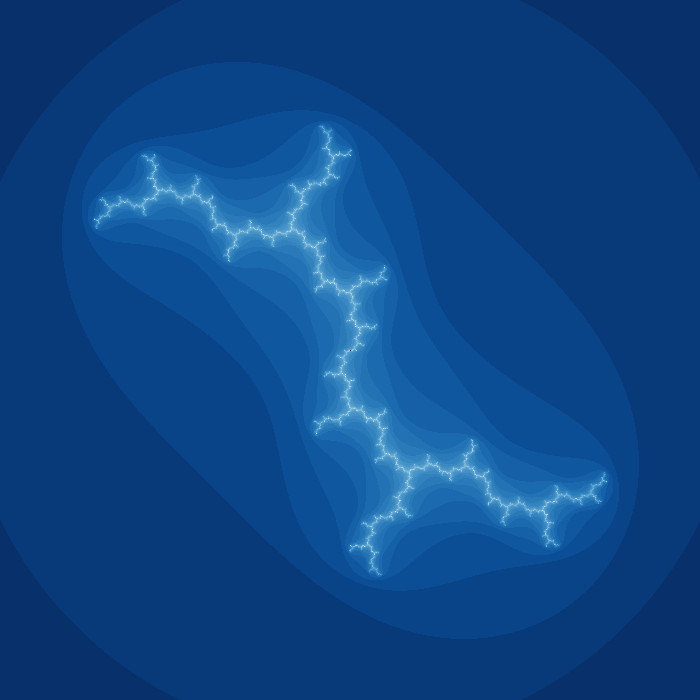
\includegraphics[scale=.4]{dendrita}
  \caption{The Julia set of $p(z) = z^2+i$, shown in white, is a dendrite.}
  \label{fig:dendrita}
\end{figure}

\begin{myexmp}[breakable]{}{ex05}
Consider the map $p(z)=z^2+(1+i/2)$. We will show that its finite critical point $z=0$ belongs to $D_\infty$. Define $g(z) = |z|-|(1+i/2)/z|$. As in the proof of Proposition \ref{pr:polyinfinite} we will find an $r_0>1$ such that $|z|\geq r_0$ implies $g(z)>2$. Let $r_0=5$, then for $|z|\geq 5$ we have
\begin{align*}
|z|-|(1+i/2)/z| &\geq 5 - \sqrt{5}/10>2.
\end{align*}
It follows that if $|p^n(z)|\geq 5$ for some $n\geq 0$ then $z\in D_\infty$. Particularly, $p^2(0) = p(1+i/2) = 7/4+i3/2$ and $p^3(0) = 29/16 + i 23/4$, so $|p^3(0)| = \sqrt{(29/16)^2+(5+3/4)^2}>5$, therefore $0\in D_\infty$. From Theorem \ref{th:TheoremfilledJulia} we deduce that $K(p)$ and $J(p)$ have uncountably many components, see Figure \ref{fig:nodendrita}. 
\end{myexmp}

\begin{figure}[h!]
	\centering
  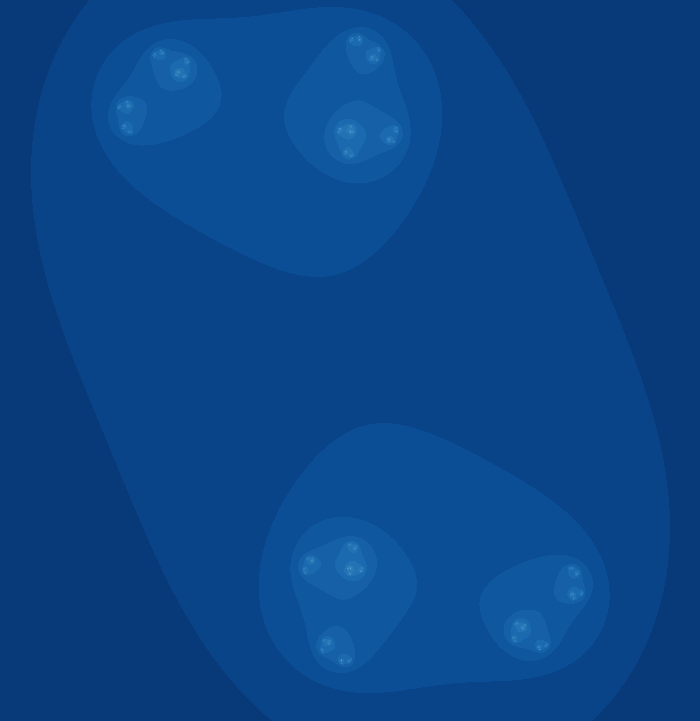
\includegraphics[scale=.4]{notdendrite}
  \caption{The white points in the image represent the Julia set of $p(z) = z^2+(1+i/2)$.}
  \label{fig:nodendrita}
\end{figure}

\section{Potential theory}

This section is intended to introduce the most important concepts and results from potential theory that we shall need. Proofs that have been omitted  can be found in \cite{ransford}, which is our main reference. A reference concerning measure theory is \cite{bartle}.\\
Let us begin by introducing the concepts of semicontinuity and subharmonic functions.
\begin{mydef}[breakable]{}{}
Let $X$ be a topological space. A function $u:X\rightarrow [-\infty,\infty)$ is said to be {\bf upper semicontinuous} if for any $\alpha\in \mathbb{R}$ the preimage $u^{-1}([-\infty,\alpha))$ is an open subset of $X$. A function $v:X\rightarrow [-\infty,\infty)$ is said to be {\bf lower semicontinuous} if $-v$ is upper semicontinuous.
\end{mydef}

\begin{mytheo}{}{upperbounded}
An upper semicontinuous $u$, defined over a topological space $X$, is bounded from above on any compact subset $K\subset X$ and attains its bound in $K$
\end{mytheo}

\begin{proof}
Since $K$ is compact, the open cover $\{ K\cap u^{-1}([-\infty,n))\}_{n\geq 1}$ must have a finite subcover, and it follows that $u$ is bounded from above on $K$. If we let $M=\sup_{x\in K}u(x)$, then $K$ cannot be covered by a finite subcollection of sets in $\mathcal{C}=\{ K\cap u^{-1}([-\infty,M-1/n))\}_{n\geq 1}$, since otherwise we would contradict the definition of $M$. By compactness of $K$, the collection $\mathcal{C}$ cannot be an open cover of $K$ and hence there must be a point $x\in K$ such that $u(x) = M$, as desired. 
\end{proof}

Subharmonic functions constitute a generalization for harmonicity. Remember that a function $v$ twice continuously differentiable and defined on an open set $D \subset \mathbb{C}$ is said to be harmonic if $\Delta v=0$, where $\Delta \coloneqq \frac{\partial^2}{\partial x^2}+\frac{\partial^2}{\partial y ^2}$ is the Laplacian operator.\nomenclature[12]{$\Delta$}{The Laplacian} It can be shown that over simply connected domains a harmonic function is the real part of a holomorphic function \cite[Theorem 1.1.2]{ransford}. Particularly, since open disks are simply connected, Cauchy's integral formula implies that, for fixed $a\in D$ and $r>0$ small enough such that the open disk $\{a+\rho e^{i\theta}\,:\, 0\leq \rho<r,\, \theta\in [0,2\pi]\}$ is contained in $D$, any harmonic function $v$ whose domain of definition contains this circle must satisfy the Mean Value Property, namely
\begin{equation}\label{harmonicity}
v(a) = \frac{1}{2\pi} \int_{0}^{2\pi} \,v(a+re^{i\theta})\,d\theta.
\end{equation}
Subharmonic functions are a generalization of harmonic functions, we now provide its definition.

\begin{mydef}{}{subharmonic}
Let $D\subset \mathbb{C}$ be an open set. A function $u:D \rightarrow [-\infty,\infty)$ is said to be {\bf subharmonic} if it is upper semicontinuous and for any $a\in D$ there exists $\rho>0$ such that
\begin{equation}\label{localsubmean}
u(a) \leq  \frac{1}{2\pi} \int_{0}^{2\pi} \,u(a+re^{i\theta})\,d\theta, \qquad \forall \,0\leq r < \rho.
\end{equation}
\end{mydef}

The inequality given in \eqref{localsubmean} is known as {\bf local submean inequality}. Notice that if $u$ is upper semicontinuous then $u^+(z)=\max\{u(z),0\}$ is bounded from above on compact sets and hence $u^+$ is integrable. Therefore, the integral of $u$ given in $\eqref{localsubmean}$ is well defined although it could be $-\infty$. Notice that if $u(z)=-\infty$ for some $z$ then \eqref{localsubmean} is satisfied trivially on sufficiently small circumferences around $z$.\\

\begin{myprop}{}{limsupequal}
If $u$ is subharmonic on an open set $D\subset \mathbb{C}$, then
$$\limsup_{z\rightarrow \zeta} u(z) =u(\zeta), \qquad \text{ for all } \zeta\in D.$$
\end{myprop}

\begin{proof}
Upper semicontinuity implies $\limsup_{z\rightarrow \zeta} u(z) \leq u(\zeta)$. However, an strict inequality is impossible since $u$ must satisfy the local submean inequality \eqref{localsubmean}.
\end{proof}

As a consequence of classical limit theorems for Lebesgue integrals we have the next proposition.

\begin{myprop}{}{decreasingsubharmonics}
Let $\{u_n\}_{n\geq 1}$ be a decreasing sequence of subharmonic functions defined on some open set $D\subset \mathbb{C}$, that is $u_n(z)\geq u_{n+1}(z)$ for all $n\geq 1$ and $z\in D$, then $u=\lim_{n\rightarrow \infty}u_n$ is a subharmonic function defined on $D$.
\end{myprop}

\begin{proof}
We need to check that $u$ is upper semicontinuous. Let $\alpha\in \mathbb{R}$ then $u(z)<\alpha$ if and only if there is some $n_0\geq 1$ such that $u_{n_0}(z)<\alpha$, hence $u^{-1}([-\infty,\alpha)) = \cup_{n\geq 1} u_n^{-1}([-\infty,\alpha))$ and evidently the righthand side is open. Since $\alpha$ is any number we conclude that $u$ is upper semicontinuous. Up to addition by a constant, we may suppose that $0 \geq u_1(z) \geq u_2(z) \geq \cdots \geq u_n(z) \geq \cdots$ on any compact set. Then, the Monotone Convergence Theorem implies
$$\lim_{n\rightarrow \infty}\int_0^{2\pi} u_n(a+re^{i\theta})\,d\theta = \int_0^{2\pi} u(a+re^{i\theta})\,d\theta,$$
whence
$$u(a) =\lim_{n\rightarrow \infty}u_n(a) \leq \lim_{n\rightarrow \infty} \frac{1}{2\pi} \int_0^{2\pi} u_n(a+re^{i\theta})\,d\theta = \frac{1}{2\pi} \int_0^{2\pi} u(a+re^{i\theta})\,d\theta,$$ 
for $a\in D$ and $r$ small enough as stated before. We conclude that $u$ is subharmonic.
\end{proof}

By the Cauchy-Riemann equations the real part of a holomorphic function is harmonic. In the case of subharmonic function we have the following.

\begin{mytheo}{}{log-subharmonic}
If $f$ is a holomorphic function on an open set $D\subset \mathbb{C}$, then $\log|f|$ is subharmonic on $D$.
\end{mytheo}

\begin{proof}
Let $u(z) = \log|f(z)|$, then $u^{-1}([-\infty,\alpha)) = \{z\,:\, |f(z)| < e^{\alpha}\}$ is open for any $\alpha\in \mathbb{R}$, hence $u$ is upper semicontinuous. Also, if $f(a)\neq 0$ for $a\in D$, then $u$ is harmonic near $a$ and hence satisfies \eqref{harmonicity}. On the other hand if $f(a)=0$ said after Definition \ref{df:subharmonic} that $u$ is trivially subharmonic at $a$. The proof is finished.
\end{proof}

Non-constant subharmonic functions, as  non-constant holomorphic and harmonic functions, satisfy a maximum principle: they do not attain global maxima at the interior of a domain. Also, as it is detailed below, if the values of $u$ are bounded near the boundary of a domain, such bound holds for every point contained in the interior of the whole domain. 

\begin{mytheo}{Maximum Principle}{maximumsubharmonic}
Suppose $u$ is a subharmonic function on a domain $D\subset \mathbb{C}$.
\begin{enumerate}
\item [(a)] If $u$ attains a global maximum on $D$, then $u$ must be a constant.\\
\item [(b)] If $\limsup_{z\rightarrow \zeta}u(z) \leq 0$ for all $\zeta\in \partial D$, then $u\leq 0$ on $D$.
\end{enumerate}
\end{mytheo}

\begin{proof}
\begin{enumerate}
\item [a)] Let $M$ be a global maximum for $u$ on $D$. Let $A=\{z\in D\,:\,u(z)<M$ and $B=\{z\in D\,:\,u(z)=M\}$. The set $A$ is open by upper semicontinuity of $u$. The set $B$ is also open, since if $u(\zeta)=M$ then \eqref{localsubmean} implies that $u$ must be equal to $M$ on all sufficiently small circles around $\zeta$. Since $D$ is connected and $B$ is non-empty by assumption, one gets that $D=B$ hence $u$ is constant.
\item [b)] For this case, we need to consider $D$ as a subset of $\widehat{\mathbb{C}}$. If we extend $u$ to $\partial D$ by defining $u(\zeta) = \limsup_{z\rightarrow \zeta}u(z)$ for all $\zeta\in \partial D\subset \widehat{\mathbb{C}}$, then $u$ is upper semicontinuous on $\overline{D}$, which is a compact set, hence $u$ attains some global maximum on it. If such maximum occurs in $\partial D$, the conclusion follows, otherwise by part (a) $u$ is constant and we achieve also the conclusion. 
\end{enumerate}
\end{proof}

Subharmonic functions have many interesting properties, just to mention one they are locally integrable: that is, if $u$ is a subharmonic function not identically $-\infty$ defined on a domain $D\subset \mathbb{C}$ then for each compact subset $K\subset D$ we have $\int_K|u|\,dA<\infty$, where $dA$ denotes the Lebesgue area measure \cite[Theorem 2.5.1]{ransford}. As a consequence of this, by taking an exhaustion of $D$, one can deduce that $\{z\in D\,:\, u(z)=-\infty\}$ is a set of Lebesgue measure zero \cite[Corollary 2.5.3]{ransford}.\\

We are now ready to introduce some potential theory notions.

\begin{mydef}{}{potential}
Let $\mu$ be a finite Borel measure on $\mathbb{C}$ with compact support. Then we define its {\bf logarithmic potential} as the function $p_\mu:\mathbb{C} \rightarrow [-\infty,\infty)$ given by
$$p_\mu(z) = \int_{\mathbb{C}} \log|z-w|\,d\mu(w).$$ \nomenclature[13]{$p_\mu$}{The logarithmic potential of $\mu$}
\end{mydef}

We know from Theorem \ref{th:log-subharmonic} that for fixed $w\in \mathbb{C}$ the function $z\mapsto \log|z-w|$ is subharmonic, hence we could expect that $p_\mu(z)$ is still a subharmonic function, and indeed it is. However we shall need the following technical result in order to provide a formal proof.

\begin{mytheo}{}{conditionsubha}
Let $(\Omega,\mu)$ be a measure space with $\mu(\Omega)<\infty$, let $U\subset \mathbb{C}$ be an open subset, and let $v:U\times \Omega \rightarrow [-\infty,\infty)$ be a function such that
\begin{enumerate}
\item[(a)] $v$ is measurable on $U\times \Omega$;\\
\item[(b)] $z\mapsto v(z,w)$ is subharmonic on $U$ for each $w\in \Omega$;\\
\item[(c)] $\zeta \mapsto \sup_{w\in \Omega} v(\zeta,w)$ is locally bounded above on $U$.
\end{enumerate}
Then $u(z)\coloneqq \int_\Omega v(z,w)\,d\mu(w)$ is subharmonic on $U$.
\end{mytheo}

\begin{proof}
Since subharmonicity is a local property it is sufficient to prove that $u$ is subharmonic on each relatively compact subdomain $D$ of $U$. If $D$ is any such subdomain, by (c) $\sup_w v(z,w)$ is bounded above on $D$, so by subtracting an adequate constant we may suppose that $v\leq 0$ on $D\times \Omega$.\\

Now, if $z_n\rightarrow z$ in $D$, by Fatou's Lemma
$$\int_\Omega \liminf_{n\rightarrow \infty} -v(z_n,w)\,d\mu(w) \leq \liminf_{n\rightarrow \infty} -u(z_n),$$
hence
$$\limsup_{n\rightarrow \infty} u(z_n) \leq \int_\Omega \limsup_{n\rightarrow \infty} v(z_n,w)\,d\mu(w).$$
But by upper semicontinuity of $\zeta \mapsto v(\zeta,w)$ given in (b) we have
$$ \int_\Omega \limsup_{n\rightarrow \infty} v(z_n,w)\,d\mu(w) \leq \int_\Omega v(z,w) \,d\mu(w)=u(w),$$
hence $u$ is upper semicontinuous on $D$.\\

Now let $z\in D$ and take $\rho>0$ small enough such that $\{z+r e^{i\theta}\,:\, 0\leq r\leq \rho,\, \theta\in[0,2\pi)\} \subset D$, then by Tonelli's theorem \cite[Theorem 10.9]{bartle} applied to $-v$ and by (b) we get
\begin{align*}
\frac{1}{2\pi} \int_0^{2\pi} u(z+\rho e^{i\theta})\,d\theta &= \int_\Omega \left( \frac{1}{2\pi} \int_0^{2\pi} v(z+\rho e^{i\theta},w)\,d\theta \right) d\mu(w)\\
&\geq \int_\Omega v(z,w)\,d\mu(w) = u(w).
\end{align*}
Therefore $u$ satisfies the submean inequality on $D$.
\end{proof}

Recall that the {\it support of a measure} $\mu$ on a topological space $X$, is given by $\supp(\mu)=\{x\in X\,:\, \mu(U)>0 \text{ for every neighborhood } U \text{ of } x\}.$ It can be proven that if $X$ has a countable base of open sets, then $\supp\,\mu$ is the smallest closed subset $F\subset X$ such that $\mu(X\setminus F)=0$, see \cite[Theorem A.1.2]{ransford}.\\

\begin{mytheo}{}{propertypotential}
Let $\mu$ be finite Borel measure on $\C$ with compact support. Then the potential $p_\mu$ is a subharmonic function on $\mathbb{C}$, and harmonic on $\mathbb{C}\setminus \supp(\mu)$.
\end{mytheo}

\begin{proof}
We can consider $\mu$ as a measure on $K\coloneqq \supp(\mu)$. It is straightforward to check that $v(z,w) = \log|z-w|$ satisfies the hypothesis of Theorem \ref{th:conditionsubha} on $\mathbb{C}\times K$, from which it follows that $p_\mu$ is subharmonic. Applying the same theorem to $v(z,w)=-\log|z-w|$ on $(\mathbb{C}\setminus K)\times K$ we get that $p_\mu$ is superharmonic on $\mathbb{C}\setminus K$, hence harmonic there.
\end{proof}

\begin{mydef}{}{}
Let $\mu$ be a finite Borel measure on $\mathbb{C}$ with compact support. We define its {\bf energy} $I(\mu)$ by
$$I(\mu) \coloneqq \int \int \log|z-w|\,d\mu(z)\,d\mu(w) = \int p_\mu(z) \,d\mu(z).$$ \nomenclature[14]{$I(\mu)$}{The energy of $\mu$}
\end{mydef}

\begin{mydef}{}{nearlyeverywhere}
\begin{itemize}
\item[ (a)] We say that a subset $E\subset \mathbb{C}$ is {\bf polar} if $I(\mu)=-\infty$ for every finite Borel measure $\mu \neq 0$ such that $\supp(\mu)$ is compact and contained in $E$.\\
\item [(b)] A property holds {\bf nearly everywhere} on a subset $S$ of $\mathbb{C}$ if it holds everywhere on $S\setminus E$, where $E$ is a Borel polar set.
\end{itemize}
\end{mydef}

It is known that if $\mu$ has finite energy and $E\subset \mathbb{C}$ is any Borel polar set, then $\mu(E)=0$ \cite[Theorem 3.2.3]{ransford}. Particularly, one can deduce that every Borel polar set has Lebesgue measure zero \cite[Corollary 3.2.4]{ransford}.

\begin{mydef}{}{}
Given $K\subset \mathbb{C}$ compact, denote by $\mathcal{P}(K)$ the set of all Borel probability measures on $K$. If there exists $\nu\in \mathcal{P}(K)$ such that
$$I(\nu) = \sup_{\mu \in \mathcal{P}(K)} I(\mu),$$
then $\nu$ is called an {\bf equilibrium measure} for $K$.
\end{mydef} 

Consider a topological space $X$, and denote by $C_c(X)$ the vector space of continuous functions with compact support $\phi:X\rightarrow \mathbb{R}$. It is known by the Riesz Representation Theorem \cite[Theorem A.3.2]{ransford} that for every continuous linear functional $\Lambda$ on $C_c(X)$ there is a unique Radon measure (a Borel measure which is finite when evaluated on every compact subset of $X$) such that
\begin{equation}\label{Rieszrelation}
\Lambda(\phi) = \int_X\,\phi\,d\mu.
\end{equation}

Denote by $C(X)$ the space of continuous functions $\phi:X\rightarrow \mathbb
{R}$ equipped with the supremum norm, let $\mathcal{P}(X)$ be the set of probability measures on $X$. A sequence $\{\mu_n\}_{n\geq 1}\subset \mathcal{P}(X)$ is $\text{weak}^*$-convergent to $\mu\in \mathcal{P}(X)$ if for every $\phi\in C(X)$ the condition
$$\lim_{n\rightarrow \infty} \int_X \phi\,d\mu_n = \int_X \phi\,d\mu,$$ 
holds. In this case we write $\mu_n \overset{w^*}{\to} \mu$. Using relation \eqref{Rieszrelation} and the notion of wea$\text{k}^*$ topology one can deduce that every compact subset $K\subset \mathbb{C}$ has an equilibrium measure \cite[Theorem 3.3.2]{ransford}. It is known that uniqueness for the equilibrium measure holds in compact non-polar subsets of $\mathbb{C}$ \cite[Theorem 3.7.6]{ransford}.

\begin{mytheo}{}{unicidadequilibrio}
For each $K$ compact non-polar subset of $\mathbb{C}$ there exists a unique equilibrium measure. Moreover, if $\nu$ is the equilibrium measure for $K$ then $\supp(\nu) \subset\partial_e K$, where $\partial_e K$ denotes the boundary of the unbounded component of $\mathbb{C}\setminus K$.
\end{mytheo}

Now we state the so called Fundamental Theorem of Potential Theory, better known as Frostman's Theorem, which in a certain sense justifies why the equilibrium measure is given such a name.

\begin{mytheo}{}{frostman}
Let $K$ be a compact set in $\mathbb{C}$ and $\nu$ an equilibrium measure for $K$. Then
\begin{itemize}
\item[(a)] $p_\nu(z) \geq I(\nu)$ for all $z\in \mathbb{C}$.\\
\item[(b)] $p_\nu(z)=I(\nu)$ on $K\setminus E$, where $E$ is a countable union of closed polar subsets of $\partial K$.
\end{itemize}
\end{mytheo}

We shall not give the proof of Theorem \ref{th:frostman} but we prove the following proposition which, although trivial, is stated for future use. Notice that Frostman's Theorem is a kind of converse for this proposition.

\begin{myprop}{}{almostequilibrium}
Let $K\subset \mathbb{C}$ be a compact subset. Suppose there is a measure $\mu$ supported in $K$ and that $p_\mu(z) \geq I(\nu)$ for all $z\in \mathbb{C}$, where $\nu$ is an equilibrium measure for $K$. Then $\mu$ is also an equilibrium measure.
\end{myprop}
\begin{proof}
Since $\mu$ is a probability measure it follows that
$$I(\mu)=\int p_\mu(z)\,d\mu(z) \geq \int I(\nu)\,d\mu(z)=I(\nu).$$
But by definition of the equilibrium measure, we actually have $I(\mu)=I(\nu)$. Therefore $\mu$ is an equilibrium measure.
\end{proof}


Now we prove the following relation for the potentials of a weak$^*$-convergent sequence of measures.\\

\begin{myprop}{}{weakconvergencep}
Let $K\subset \mathbb{C}$ be a compact subset. If $\mu_n \overset{w^*}{\rightarrow} \mu$ where all measures are in $\mathcal{P}(K)$, then it follows that
$$\limsup_{n\rightarrow \infty} p_{\mu_n}(z) \leq p_{\mu}(z), \quad \text{ for all } z\in \mathbb{C}.$$
\end{myprop}

\begin{proof}
Notice that for a fixed $z\in \mathbb{C}$  and each $m\geq 1$ the function $w\mapsto \max\{\log|z-w|,-m\}$ is continuous in $\mathbb{C}$. Hence
\begin{align*}
\limsup_{n\rightarrow \infty} p_{\mu_n}(z) &= \limsup_{n\rightarrow \infty} \int_K \log|z-w| \,d\mu_n(w)\\
&\leq \limsup_{n\rightarrow \infty} \int_K \max\{\log|z-w|,-m\} \,d\mu_n(w)\\
&= \int_K \max\{\log|z-w|,-m\} \,d\mu(w).
\end{align*}
By taking the limit when $m\rightarrow \infty$ in the previous inequality and by the Monotone Convergence Theorem we deduce $\limsup_{n\rightarrow \infty} p_{\mu_n}(z) \leq p_{\mu}(z).$
\end{proof}

The last notion we are going to introduce in this section, and also very useful, is that of capacity. Recall that if $X$ is a toplogical space, then $A\subset X$ is said to be {\it relatively compact} if the closure of $A$ is a compact subset of $X$, in this case we write $A\subset\subset X$.

\begin{mydef}{}{}
The (logarithmic) {\bf capacity} of a subset $E$ of $\mathbb{C}$ is given by
$$c(E) \coloneqq \sup \{e^{I(\mu)}\,:\, \supp(\mu)\subset \subset E \text{ and } \mu \text{ is a probability measure on } \mathbb{C}\}.$$ \nomenclature[15]{$c(E)$}{The capacity of $E$}
\end{mydef}

Since the support of a measure is always a closed subset, $\supp(\mu)\subset \subset E$ implies that $\supp(\mu)$ is compact. Notice that if $K$ is compact and $\nu$ is an equilibrium measure for $K$ then $c(K) = e^{I(\nu)}$. Also, under the convention $e^{-\infty}=0$ it follows that $c(E)=0$ if and only if $E$ is a polar subset. Basic properties of capacity are given in the following theorem.\\

\begin{mytheo}{}{teoinvcap}
\begin{enumerate}
\item[(a)] Let $T(z)=az+b$ for $a,b\in \mathbb{C}$. Then, if $E\subset \mathbb{C}$ we have $c(T(E)) = |a|c(E)$.\\
\item[(b)] If $K\subset \mathbb{C}$ is a compact subset then $c(K) = c(\partial_e K)$.\\
\end{enumerate}
\end{mytheo}

\begin{proof}
To prove (a), notice that the result is straightforward for $a=0$. Hence, suppose $a\neq 0$ and let $T:\mathbb{C} \rightarrow \mathbb{C}$ be defined as $T(z) = az+b$. Let $\mu$ be a probability measure such that $\supp \,\mu \subset E$. The {\it push-forward} measure $T_*\mu$ is defined by $T_*\mu(A) = \mu(T^{-1}(A))$ for every Borel set $A\subset \mathbb{C}$. \nomenclature[16]{$T_*\mu$}{The push-forward measure of $\mu$ by $T$} It follows that $\supp \, T_*\mu \subset T(E)$. Also,
\begin{align*}
\int_{T(E)}\int_{T(E)} \log|z-w|\,dT_*\mu(z)dT_*\mu(w) &= \int_{E}\int_{E} \log|T(z)-T(w)| \,d\mu(z)d\mu(w).\\
&= \log|a|+I(\mu),
\end{align*}
where we have used that $\mu(E)=1$ in the last equality.\\

This shows that $c(T(E)) \geq |a|c(E)$. Using $T^{-1}:T(E)\rightarrow E$, the same argument implies that $c(T(E)) = |a|c(E)$.\\

Finally, (b) is a direct consequence of Theorem \ref{th:unicidadequilibrio}.\\

\end{proof}

The capacity of the Julia set can be explicitly calculated for polynomials.

\begin{mytheo}{}{capacitypolyno}
If $p(z) = \sum_{j=0}^da_jz^j$ is a polynomial of degree $d\geq 2$, then its Julia set has capacity $c(J(p)) = 1/|a_d|^{1/(d-1)}$
\end{mytheo}

\begin{proof}
For the proof we need the following two technical properties of capacity, the proofs can be found in \cite{ransford}.

\begin{enumerate}
\item Let $K\subset \mathbb{C}$ be a compact set and let $p(z)$ be a polynomial of degree $d\geq 1$. Then
$$c(p^{-1}(K)) = \left( \frac{c(K)}{|a_d|}\right)^{1/d}.$$ 
\item If $K_1 \supset K_2 \supset K_3\supset \cdots$ are compact subsets of $\mathbb{C}$ and $K = \cap_{n\geq 1} K_n$, then 
$$c(K) = \lim_{n\rightarrow \infty} c(K_n).$$
\end{enumerate}

Now let $p$ be a monic polynomial of degree $d\geq 2$. There is an $R>0$ such that $|p(z)|\geq 2|z|$ when $|z|>R$, define $U= \{z\in \mathbb{C}\,:\, |z|>R\}$. Notice that $p^{-n}(U)= \{ z\in \mathbb{C}\,:\, p^n(z)\in U\} \supset U$ for each $n\geq 0$. Now define $K_n = \C \setminus p^{-n}(U)$, it follows that $K_n = p^{-1}(K_{n-1})$ for each $n$, so 
$$c(K_n) = c(K_{n-1})^{1/d} = c(K_{n-2})^{1/d^2}= \cdots = c(K_0)^{1/d^n}.$$ 
Also, it is easy to check that if $K = \C\setminus(\cup_{n\geq 1} p^{-n}(U))$ then $K = \bigcap_{n\geq 1} K_n $, so 
$$c(K) = \lim_{n\rightarrow \infty} c(K_n) = \lim_{n\rightarrow \infty} c(K_0)^{1/d^n} = 1.$$
Since $D_\infty = \cup_{n\geq 1} p^{-n}(U)$ we have $\partial K = \partial D_\infty = J(f)$. But $c(K) = c(\partial K)$ by Theorem \ref{th:teoinvcap} (b), so $c(J(p))=1$ and the result follows when $p$ is monic polynomial.\\

Now, suppose that $p(z) = a_dz^d+\cdots + a_0$. Let $m(z) = a_d^{1/(d-1)}z$, it is easy to check that $q(z) = m\circ p\circ m^{-1}$ is monic. By the previous case $c(J(q))=1$, so $C(J(p))=1/|a_d|^{1/(d-1)}$ by Theorems \ref{pr:conjugation} and \ref{th:teoinvcap} (a).
\end{proof}
%In order to give a proof for Theorem \ref{th:capacitypolyno} we need to introduce the concept of Green function.

\subsection{The Green function and its relation to complex dynamics}\label{subsectionn}

\begin{mydef}{}{green_potencial_def}
Let $D\subset \C$ be a domain containing $\infty$. A {\bf Green function} with pole at $\infty$ for $D$ is a function $g_D(\cdot,\infty):D \rightarrow (-\infty,\infty]$ such that for each $w \in D$:\nomenclature[16]{$g_D(\cdot,\infty)$}{The Green function with pole at $\infty$ for $D$}
\begin{itemize}
\item[(a)] $z\mapsto g_D(\cdot,\infty)$ is harmonic on $D\setminus \{\infty\}$ and bounded on the complement of each neighborhood of $\infty$;\\
\item[(b)] $g_D(\infty,\infty) = \infty$ and
$g_D(z,\infty) = \log|z|+O(1),$
as $z\rightarrow \infty$;\\
\item[(c)] $g_D(z,\infty) \rightarrow 0$ as $z \rightarrow \zeta$  for nearly every $\zeta\in \partial D$. 
\end{itemize} 
\end{mydef}

Notice that a Green function $G_D$ may be defined as identically $0$ on $\C\setminus D$, and then it would be defined on the whole $\C$. We can prove existence of the Green function for arbitrary domains with non-polar boundary. For this, we need to make use of the {\bf Extended Maximum Principle} for subharmonic functions. 

\begin{mytheo}{}{extended maximum}
Let $D$ be a domain in $\mathbb{C}$, and let $u$ be a subharmonic function on $D$ which is bounded above. If $\partial D$ is non-polar and $\limsup_{z\rightarrow \zeta} u(z)\leq 0$ for nearly every $\zeta \in \partial D$, then $u\leq 0$ on $D$. 
\end{mytheo}

A proof of Theorem \ref{th:extended maximum} can be found in \cite[Theorem 3.6.9]{ransford}.\\

\begin{mytheo}{}{existencefuncgreen}
Let $D\subset \C$ be a domain whose boundary is non-polar, then there exists a unique Green function $g_D(z,\infty)$ for $D$.
\end{mytheo}

\begin{proof}
Let us address uniqueness first. Suppose that $g_1(z,\infty)$ and $g_2(z,\infty)$ are two Green functions for $D$. Define $h(z)=g_1(z,\infty)-g_2(z,\infty)$. Then $h$ is harmonic and bounded on $D\setminus\{\infty\}$. Actually, $\lim_{z\rightarrow \zeta}h(z) = 0$ for nearly every $\zeta\in \partial D$, so this limit holds almost everywhere in $\partial D$. With the intention of applying the Maximum Principle for harmonic functions, $h$ may be extended continuously to $\C\setminus D$, defining it as identically $0$ on $\C \setminus D$. However, this is not sufficient to conclude that $h\leq 0$ on $D$, since near $\infty$ the function $h$ tends to a constant which in principle may be greater than $0$. However, by Theorem \ref{th:extended maximum} we can conclude that $h\leq 0$ on $D$. Applying the same argument to $-h$ we deduce that actually $h\equiv 0$. Hence the Green function is unique.\\

To show existence, define
$$g_D(z,\infty) = \begin{cases}
p_\nu(z)-I(\nu), & z\in D\setminus\{\infty\},\\
\infty, & z=\infty,
\end{cases}.$$
where $\nu$ is the equilibrium measure for $\C\setminus D$. Since,
$$p_\nu(z) = \log|z| + \int \log|1-w/z|\,d\nu(w),$$
and $\log|1-w/z|\,d\nu(w)$ tends to $0$ as $z\rightarrow \infty$, it follows that $p_\nu(z)-I(\nu) = \log|z| + O(1)$ as $z\rightarrow \infty$. The rest of the properties are direct consequences of Theorems \ref{th:propertypotential} and \ref{th:frostman}.
\end{proof}

As a consequence of Theorem \ref{th:existencefuncgreen}, for a non-constant polynomial $p$ of degree $d\geq 2$ the attracting basin $D_\infty$ has a Green function. Indeed, for such a polynomial by Theorem \ref{th:capacitypolyno} the set $J(f)=\partial D_\infty$ is non-polar. It turns out that the Green function has important properties related to the dynamics of the given polynomial.\\

\begin{mytheo}{}{teogreenpoli}
Let $p(z)=\sum_{j=0}^da_jz^j$ be a polynomial of degree $d\geq 2$, and $D_\infty$ the attracting basin of $\infty$ for $p$. Then
$$g_{D_\infty}(p(z),\infty) = d g_{D_\infty}(z,\infty), \quad \,\text{ for }z\in D_\infty.$$
\end{mytheo}

\begin{proof}[Proof of Theorem \ref{th:teogreenpoli}]
Let $D=D_\infty\setminus \{\infty\}$ and define $h:D \rightarrow \mathbb{R}$ by
$$h(z) = g_{D_\infty}(p(z),\infty)-dg_{D_\infty}(z,\infty).$$
It can be checked that composition of an analytic function with a harmonic function is also harmonic, so $h$ is harmonic on $D$. Also, $h$ is bounded for $z$ outside a neighborhood of $\infty$, by definition of the Green function and the fact that if $U$ is a neighborhood of $\infty$, and $K=\C \setminus U$, then $\C \setminus p(K)$ is also a neighborhood of $\infty$. On the other hand, as $z\rightarrow \infty$,
$$h(z) = \log|p(z)|-d\log |z|+O(1)=\log|p(z)/z^d|+O(1)=O(1),$$
that is, $h(z)$ is bounded for $|z|$ sufficiently large. We conclude that $h$ is bounded on $D$.\\

Now, if $w=p(\zeta)$ for some $\zeta\in \partial D_\infty$, then $w\in \partial D_\infty$. Also, notice that $g_{D_\infty}(p(z),\infty) \rightarrow 0$ as $z\rightarrow \zeta$ if and only if $g_{D_\infty}(w,\infty) \rightarrow 0$ as $w\rightarrow p(\zeta)$. Hence $h(z) \rightarrow 0$ as $z\rightarrow \zeta$ for nearly every $\zeta \in \partial D_\infty$. This implies that $h(z) \leq 0$ for nearly every $\zeta \in \partial D= \partial D_\infty \cup \{\infty\}$. We apply now Theorem \ref{th:extended maximum} to conclude that $h\leq 0$ on $D$. But exactly the same arguments may be applied to $-h$ to obtain $-h \leq 0$, so necessarily $h\equiv 0$, and the theorem follows.
\end{proof}

\begin{mydef}{}{}
Let $D\subset \C$ be a proper subdomain and $\zeta_0\in \partial D$. A {\bf barrier} at $\zeta_0$ is a subharmonic function $u$ defined on $D\cap N$, where $N$ is an open neighborhood of $\zeta_0$, satisfying
$$u<0 \text{ on } D\cap N \quad \text{and} \quad \lim_{z\rightarrow \zeta_0} u(z_0)=0.$$
If there is a barrier at $\zeta_0$, then this point is called {\bf regular}, otherwise it is {\bf irregular}. The domain $D$ is called {\bf regular} if every point at its boundary is regular. 
\end{mydef}

\begin{mytheo}{}{}
If $D\subset \C$ is a simply connected domain such that $\C\setminus D$ contains at least two points, then $D$ is a regular domain.
\end{mytheo}

\begin{proof}
Let $\zeta_0\in \partial D$, we need to show that there exists a barrier at $\zeta_0$. Choose $\zeta_1\in \partial D\setminus\{z_0\}$. Under conjugation by a Möbius transformation we may suppose that $\zeta_0=0$ and $\zeta_1=\infty$. Then $D$ is a simply connected domain contained in $\mathbb{C}\setminus\{0\}$. Thereby, there is a holomorphic branch of $\log z$ on $D$. Let $N=\{|z|<1\}$ and define $u:N\rightarrow \mathbb{R}$ by
$$u(z) = \text{Re}(1/\log z).$$
Then certainly $u(z)<0$ on $D\cap N$ and $\lim_{z\rightarrow 0} u(z)=0$, so the theorem follows.
\end{proof}

\begin{mycoro}{}{}
Let $D$ be a subdomain of $\C$, and let $\zeta_0\in \partial D$. It $\zeta_0$ belongs to a connected component of $\partial D$ which contains a different point than $\zeta_0$, then $\zeta_0$ is a regular point of $\partial D$.
\end{mycoro}

\begin{mycoro}{}{corogreenf}
With the same hypotheses as in Theorem \ref{th:teogreenpoli}, the Green function $g_{D_\infty}(z,\infty)$ is given as
$$g_{D_\infty}(z,\infty) = \lim_{n\rightarrow \infty} \frac{\log |p^n(z)|}{d^n}.$$
\end{mycoro}

\begin{proof}
Since by definition of the Green function
$$g_{D_\infty}(z,\infty)=\log|z| + O(1),$$
as $z\rightarrow \infty$, then from Theorem \ref{th:teogreenpoli} we get
$$g_{D_\infty}(z,\infty) = d^{-n}g_{D_\infty}(p^n(z)) = d^{-n}\log|p^n(z)| + O(d^{-n}) \quad \text{as }n \rightarrow \infty.$$

Since $p^n(z) \rightarrow \infty$ locally uniformly on $D_\infty$, the previous convergence is also locally uniformly on $D_\infty$.
\end{proof}

%Now we end this section with the following proof.\\


\section{Three concepts from complex analysis in several variables}

In this section we will be interested in introducing domains of holomorphy, holomorphically convex sets and pseudoconvexity. We will see below that these are equivalent concepts. We need this theory to state and prove some properties found in Proposition \ref{pr:pesudo_homo}, regarding the basin of attraction of the origin for a homogeneous polynomial. However, the content of this section is not essential for further developements in subsequent chapters.\\

Through this section $\Omega$ will always denote an open subset of $\mathbb{C}^n$ where $n\geq 1$. We shall use capital letters to denote elements in $\mathbb{C}^n$. The reader may find fundamental theory of holomorphic functions of several variables in \cite{gunning} as well as in \cite{hormander}.

\begin{mydef}{}{def:holsev}
Let $\Omega \subset \mathbb{C}^n$ be an open set, a complex-valued function $f:\Omega \rightarrow \mathbb{C}$ is called {\bf holomorphic} if for each $A=(a_1,\dots,a_n)\in \Omega$, the function $f(Z)=f(z_1,z_2,\dots,z_n)$ can be represented as a convergent power series
$$\sum_{k_j \geq 0,1\leq j\leq n} c_{k_1\dots\, k_n}(z_1-a_1)^{k_1}\cdots (z_n-a_n)^{k_n},$$
for every $Z$ in a neighborhood of $A$.
\end{mydef}

\begin{mydef}{}{defi01}
A {\bf domain of holomorphy} in $\mathbb{C}^n$ is an open subset $\Omega\subset \mathbb{C}^n$ such that there exists some holomorphic function which cannot be extended holomorphically through any boundary point of $\Omega$.
\end{mydef}

\begin{figure}[h!]
  \centering
  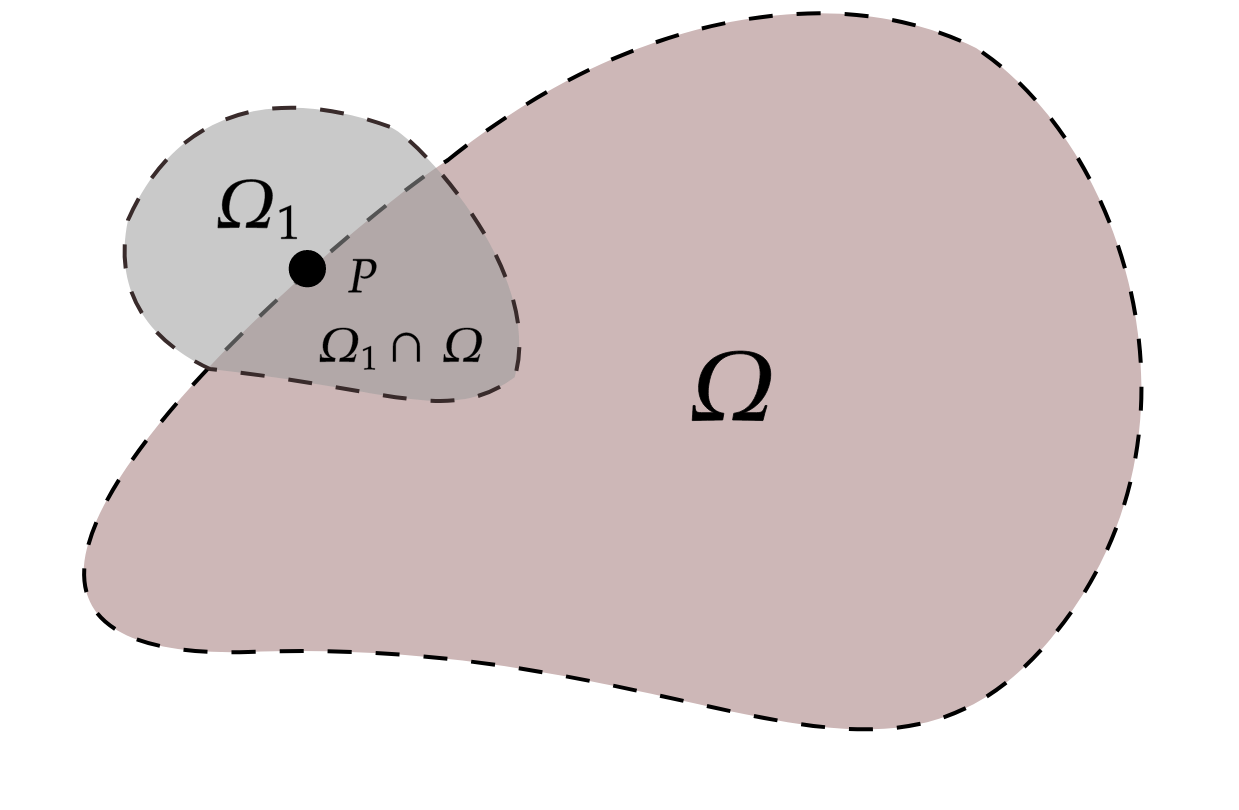
\includegraphics[scale=.2]{d001}
  \caption{In the figure $P\in \partial \Omega$ and $\Omega_1$ is a neighborhood of $P$.}
  \label{fig:dominiofront}
\end{figure}

We need to give some remarks on Definition \ref{df:defi01}. Notice that a domain of holomorphy need not be connected, as is required for domains in $\mathbb{C}$. The collection of all holomorphic functions defined on some open set $\Omega$ is denoted as $A(\Omega)$. Also, we say that an analytic function $f$ can be extended through $P\in \partial \Omega$ if there is an open set $\Omega_1\ni P$ not contained in $\Omega$ and a holomorphic function $g\in A(\Omega_1)$ such that $f=g$ on $\Omega\cap \Omega_1$, see Figure \ref{fig:dominiofront}. It is known that every domain in $\mathbb{C}$ is a domain of holomorphy \cite[Chapter G]{gunning}. However, for each $n\geq 2$, the space $\mathbb{C}^n$ contains domains which are not domains of holomorphy. The first example of such domain is due to Hartogs. We present it next, following \cite{range}.\\

\begin{figure}[h!]
  \centering
  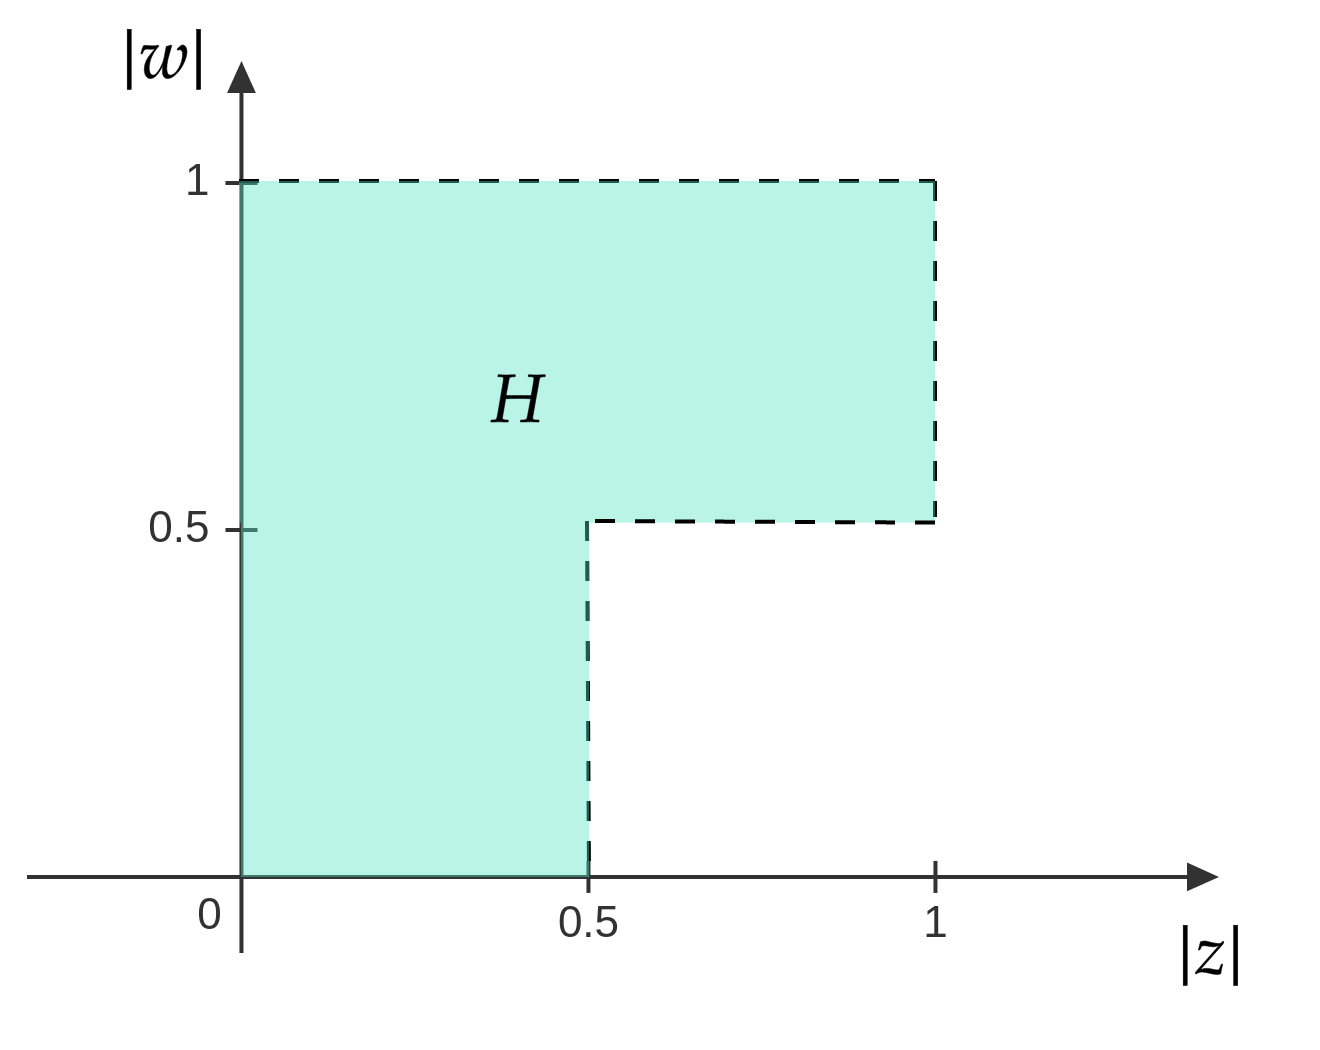
\includegraphics[scale=.2]{d002}
  \caption{A representation of Hartog's Domain.}
  \label{fig:H}
\end{figure}

\begin{myexmp}[breakable]{}{}
Consider the domain in $\mathbb{C}^2$,
$$H = \{(z,w)\,:\,|z|<1, 1/2<|w|<1\} \cup \{(z,w)\,:\,|z|<1/2, |w|<1\}.$$
Then if $1/2<r<1$ and $G_r = \{(z,w)\,:\,|z|<1, |w|<r\}$, any holomorphic function on $H$ can be extended to $H\cup G_r$ holomorphically. For if $f:H\rightarrow \mathbb{C}$ is holomorphic, then the function
$$F(z,w) = \frac{1}{2\pi} \int_{|\zeta|=r} \frac{f(z,\zeta)}{\zeta-w}\,d\zeta,$$
is holomorphic on $G_r$. Moreover, for fixed $|z|<1/2$ the function $w\mapsto f(z,w)$ is holomorphic on $\{|w|<1\}$, so Cauchy's Integral Formula implies that for $|w|<r$,
$$f(z,w) = \frac{1}{2\pi} \int_{|\zeta|=r} \frac{f(z,\zeta)}{\zeta-w}\,d\zeta = F(z,w).$$
Hence, by the Identity Theorem $f\equiv F$ on $H\cap G_r$. This proves that $F$ provides an extension of $f$ to $H\cup G_r$, hence $H$ is not a domain of holomorphy. See Figure \ref{fig:H} for a representation of $H$, notice that the modulus of the variables $z$ and $w$ are represented in the axes of the figure.
\end{myexmp}

It is very useful to use the following notion to characterize domains of holomorphy.

\begin{mydef}{}{convexhull}
Let $K$ be a compact subset of $\Omega\neq \emptyset$, then the $A(\Omega)$-hull $\widehat{K}_\Omega$ of $K$ is defined by
$$\widehat{K}_\Omega = \{Z\in \Omega\,:\, |f(Z)| \leq \sup_K |f|, \text{ for every } f\in A(\Omega)\}.$$
\end{mydef}

The set $\widehat{K}_\Omega$ is also called the {\bf holomorphically convex hull} of $K$ in $\Omega$. A few properties of $\widehat{K}_\Omega$ are given in the following list. \nomenclature[17]{$\widehat{K}_\Omega$}{The holomorphically convex hull of $K$ in $\Omega$}

\begin{enumerate}
\item $\widehat{K}_\Omega$ contains $K$, which is directly seen by definition. This also implies that $\sup_{\widehat{K}_\Omega}|f|=\sup_K |f|$ for each $f\in A(\Omega)$, so $\widehat{\widehat{K}}_\Omega$ reduces to $\widehat{K}_\Omega$. \\
\item $\widehat{K}_\Omega$ is closed and bounded in $\Omega$. It is closed by continuity of each function in $A(\Omega)$. Next, taking $f_i\in A(\Omega)$ as the projection $f_i(z_1,\dots,z_n) = z_i$, since $f_i|_K$ is bounded in $K$, the same follows for $f_i|_{\widehat{K}_\Omega}$ by definition. Because $1\leq i\leq n$ is arbitrary we get that every point in $\widehat{K}_\Omega$ has bounded components and so the holomorphically convex hull is bounded.\\

\item $\widehat{K}_\Omega$ contains every bounded component of $\Omega\setminus K$. Since every such component is bounded by a subset of $\partial K \subset K$, the Maximum Principle \cite[Theorem 4, Chapter A]{gunning} yields the property.
\end{enumerate}

\begin{mydef}{}{}
An open subset $\Omega \subset \mathbb{C}^n$ is called {\bf holomorphically convex} if for every $K\subset \Omega$ compact the set $\widehat{K}_\Omega$ is also compact.
\end{mydef}

The first characterization we shall need is given in the next theorem.

\begin{mytheo}{}{holomorphy}
A set $\Omega$ is a domain of holomorphy if and only if it is holomorphically convex.
\end{mytheo}

We shall not give a proof of Theorem \ref{th:holomorphy} (see the references cited above), but with its aid we will prove the following helpful result. The proof illustrates the characterization of a domain of holomorphy.\\

\begin{mytheo}{}{teohormander}
Let $\Omega\subset \mathbb{C}^n$ and $\Omega' \subset \mathbb{C}^m$ be domains of holomorphy, and let $u:\Omega \rightarrow \mathbb{C}^m$ be an analytic function, that is $u(Z)=(u_1(Z),\dots, u_m(Z))$ and each $u_j$ is holomorphic as in Definition \ref{df:def:holsev}.\\
Then, if
$$\Omega_u = \{Z\in \Omega \,:\, u(Z)\in \Omega'\}$$
is non-empty, it is a domain of holomorphy.
\end{mytheo}

\begin{proof}
The set $\Omega_u$ is open because $\Omega_u = u^{-1}(\Omega')$. Now let $K \subset \Omega_u$ be a compact set. Since $\Omega\supset \Omega_u$ is a domain of holomorphy then $\widehat{K}_{\Omega} \subset \Omega$ is compact, so $\widehat{K}_{\Omega_u} \subset \widehat{K}_\Omega$ is bounded. If we show that $\widehat{K}_\Omega$ is closed in $\Omega_u$ then it would be compact and the proof would be finished.\\

Notice that $u(K)$ is a compact subset of $\Omega'$ because $u$ is continuous. Then $\widehat{u(K)}_{\Omega'}$ is a compact subset of $\Omega'$. Now if $f\in A(\Omega')$ then $f\circ u\in A(\Omega)$ so for any $Z\in \widehat{K}_{\Omega_u}$ by definition we get
$$|f(u(Z))| \leq \sup_{Z\in K} |f(u(Z))| = \sup_{W\in u(K)} |f(W)|,$$
which in turn implies $u(Z)\in \widehat{K}_{\Omega'}$. By continuity of analytic functions, every point of accumulation of $\widehat{K}_{\Omega_u}$ in $\Omega$ is mapped by $u$ into $\widehat{K}_{\Omega'}\subset \Omega'$, so every such point belongs to $\Omega_u$ by definition, concluding the proof.
\end{proof}

Remember that a subset $A\subset \mathbb{C}^n$ is geometrically convex if whenever $X,Y\in A$ then $\lambda X + (1-\lambda)Y$ for every $\lambda\in[0,1]$. It is known that geometrically convex subsets of $\mathbb{C}^n$ are always domains of holomorphy, this is the content of the next theorem.\\

\begin{mytheo}{}{geoconvex}
If an open set $\Omega\subset \mathbb{C}^n$ is geometrically convex then it is a domain of holomorphy.
\end{mytheo}
\begin{proof}
Let $K\subset \Omega$ be compact. Consider the convex hull of $K$, that is, the smallest closed and convex set containing $K$, denote it by $K^*$. Since $\Omega$ is geometrically convex then $K^* \subset \Omega$. It is known that, in real vector spaces, compact convex subsets and disjoint points can be separated by closed hyperplanes given by real-valued linear functions \cite[Theorem 2.1.10]{hormanderconvex}. Hence, considering $\mathbb{R}^{2n}=\mathbb{C}^n$, for any point $W\in \partial \Omega$ there exists a linear function $l_W(X,iY)=l_W(Z)$ such that $l_W(W)=0$ and $l_W(Z)<0$ for $Z\in K^*\supset K$. By linearity we can also write  $l_W(Z) =c +\sum_{j=1}^n c_{1j}z_j+c_{2j}\overline{z}_{j}$ for some constants $c,c_{1j},c_{2j}$ . By the fact that $l_W$ is real-valued it is necessary that $c=\overline{c},c_{1j}=\overline{c_{2j}}$. Let $c_j=c_{1j}$, it follows that $l_W = \text{Re}\{c+\sum_{j=1}^n c_jz_j\}$. Now, the function $f_W(Z)=\exp\{c+\sum_{j=1}^nc_jz_j\}$ satisfies $|f_W(Z)|<a<1$ for some $a>0$ and for all $Z\in K$, while $f_W(W)=1$. By continuity there is a neighborhood $V_W$ of $W$ such that $|f_W(Z)|>a$ for $W\in V_W$. It follows that $\widehat{K}$ is disjoint from an open set containing $\partial \Omega$, hence is closed in $\Omega$, since it is bounded as remarked after Definition \ref{df:convexhull}. We conclude that $\Omega$ is holomorphically convex and so is a domain of holomorphy.
\end{proof}

We end this chapter by introducing the notion of pseudoconvexity. For this, let us define the generalization of subharmonic functions to higher dimensions.\\
\begin{mydef}{}{}
A mapping $u:\Omega \rightarrow [-\infty,+\infty)$ is a {\bf plurisubharmonic function} if $u$ is upper semicontinuous and for each $W\in \Omega$ and $Z\in \mathbb{C}^n$ the function $t\mapsto u(W+tZ)$ is subharmonic on its domain of definition.
\end{mydef}

The following proposition is a direct consequence of the previous definition and Proposition \ref{pr:decreasingsubharmonics}.

\begin{myprop}{}{decreasingpluri}
If $\{u_n\}_{n\geq 1}$ is a monotonically decreasing sequence of plurisubharmonic functions defined on $\Omega$ then $\lim_{n\rightarrow \infty} u_n$ is plurisubharmonic on $\Omega$.
\end{myprop}

We shall also need the following observation which is stated as a proposition for future reference.

\begin{myprop}{}{convergenceplurisub}
Suppose $\{u_n\}_{n\geq 1}$ is a sequence of continuous plurisubharmonic functions defined on $\Omega$ which converge uniformly to $u$ on compact subsets of $\Omega$, then $u$ is also continuous and plurisubharmonic.
\end{myprop}

\begin{proof}
Uniform convergence preserves continuity as well as the local submean inequality in Equation \ref{localsubmean}.
\end{proof}
For any open subset $\Omega\subset \mathbb{C}^n$ and any point $Z\in \Omega$ let $d_\Omega(Z) = \sup \{\varepsilon\geq 0\,:\, B(Z;\varepsilon)\subset \Omega\}$ where $B(Z;\varepsilon) = \{W\in \mathbb{C}^n\,:\, \|Z-W\|<\varepsilon\}$ is the ball given by the euclidean norm $\|Z\|\coloneqq (|z_1|^2+|z_2|^2+\cdots+|z_n|^2)^{1/2}$. \nomenclature[18]{$d_\Omega$}{distance to $\partial \Omega$}\\
%For any $R=(r_1,r_2,\dots,r_n)$ where $r_i>0$ for each $1\leq i \leq n$ the {\bf polydisc} centered at $Z\in \mathbb{C}^n$ with polyradius $R$ is defined as $\Delta(Z,R) \coloneqq \{W\in \mathbb{C}^n\,:\, |w_i-z_i|<r_i,\,i=1,\dots,n\}$. 

\begin{mydef}{}{}
An open set $\Omega$ is said to be {\bf pseudoconvex} if the function $-\log d_\Omega$ is plurisubharmonic in $\Omega$.
\end{mydef}

\begin{mytheo}{}{increasingpseudoconvex}
If $\{\Omega_n\}_{n\geq 1}$ is an increasing sequence of pseudoconvex open subsets of $\mathbb{C}^n$ then $\Omega = \cup_{n\geq 1}\Omega_n$ is also a pseudoconvex subset of $\mathbb{C}^n$.
\end{mytheo}

\begin{proof}
Since $\Omega_n\subset \Omega_{n+1}$ for every $n\geq 1$ we deduce that $d_{\Omega_n}\leq d_{\Omega_{n+1}}$ so the sequence of functions $\{-\log d_{\Omega_n}\}_{n\geq 1}$ is monotonically decreasing and 
$$\lim_{n\rightarrow \infty}-\log d_{\Omega_n}(Z)=-\log d_{\Omega}(Z).$$
Notice that the left hand makes sense since eventually $Z\in \Omega_n$ for all sufficiently large $n$. We deduce from Proposition \ref{pr:decreasingpluri} that $-\log d_{\Omega}(Z)$ is plurisubharmonic on each $\Omega_n$. Since plurisubharmonicity is a local condition and $\Omega = \cup_{n\geq 1}\Omega_n$ we deduce that $\Omega$ is pseudoconvex.
\end{proof}

We give the statement of the equivalence between pseudoconvex subsets and domains of holomorphy.\\

\begin{mytheo}{}{pseudoholo}
An open subset of $\mathbb{C}^n$ is a domain of holomorphy if and only if it is pseudoconvex.
\end{mytheo}

A proof of Therem \ref{th:pseudoholo} may be found in \cite[Theorem 4.2.8]{hormander}, but to go into this in detail would take us too far afield.\\

\section{The dynamical Green function}\label{sec:secciongreen}

Let us start with the definition of a fundamental class of mappings we shall be using in the rest of this work.\\

\begin{mydef}{}{}
A non-constant polynomial $f:\mathbb{C}^{n+1} \rightarrow \mathbb{C}$ is called {\bf homogeneous of degree} $d$ if it is a sum of algebraic terms of degree $d$. A holomorphic map $F:\mathbb{C}^{n+1} \rightarrow \mathbb{C}^{n+1}$ is said to be a {\bf homogeneous map} of degree $d$ if it can be expressed as 
$$F(Z) = (f_1(Z),f_2(Z),\dots, f_{n+1}(Z)),$$
where each $f_i$ is a homogeneous polynomial and $Z = (z_1,z_2,\dots,z_{n+1})\in \mathbb{C}^{n+1}$. A homogeneous map $F$ is called {\bf non-degenerate} if $F^{-1}(0)=\{0\}$, otherwise it is {\bf degenerate}.
\end{mydef}

Denote by $\mathbb{P}^n$ the projective space of complex lines through the origin in $\mathbb{C}^{n+1}$. There is a projection $\pi:\mathbb{C}^{n+1}\setminus\{0\}\rightarrow \mathbb{P}^n$ given by $\pi(Z) = [Z]$, where $[Z]$ is the set of points of the form $cZ$ with $c\in \mathbb{C}^*$. Homogeneous maps are very important due to the following theorem.

\begin{mytheo}{}{existencialevantamiento}
To every holomorphic map $f:\mathbb{P}^n \rightarrow \mathbb{P}^n$ there exists a non-degenerate homogeneous map $F:\mathbb{C}^{n+1}\rightarrow \mathbb{C}^{n+1}$ such that $\pi\circ F = f \circ \pi$.
\end{mytheo}

A proof of Theorem \ref{th:existencialevantamiento} can be found in \cite{fornaes}. In Appendix \ref{p1} we prove the theorem for the case $n=1$, for subsequent chapters this is the case we will be interested in. However, in this seccion the rest of results are proven for homogeneous maps on $\mathbb{C}^{n+1}$ for arbitrary $n\geq 1$, since the dimension $n$ is not significant for the arguments. The following exposition is based upon the reference \cite{ueda}.\\

\begin{mylema}{}{levant01}
Let $F: \mathbb{C}^{n+1} \rightarrow \mathbb{C}^{n+1}$ be a homogeneous map of degree $d$. Then, there exists a constant $M>0$ such that $\|F(Z)\| \leq M \|Z\|^d$ for all $Z\in \mathbb{C}^{n+1}$. In case that $F$ is non-degenerate, then there is a constant $m>0$ such that $\|F(Z)\| \geq m \|Z\|^d$ for all $Z\in \mathbb{C}^{n+1}$. 
\end{mylema}

\begin{proof}
If we let $M = \sup_{\|Z\|=1} \|F(Z)\|$, using that $F$ is a homogeneous map of degree $d$ we get
$$\| F(Z)\|  = \|Z\|^d \| F(Z/\|Z\|) \| \leq M \|Z\|^d.$$

Similarly, if $F$ is non-degenerate we can assure that $0<m = \inf_{\|Z\|=1} \|F(Z)\|$ and so
$$\| F(Z)\|  = \|Z\|^d \| F(Z/\|Z\|) \| \geq m \|Z\|^d.$$
\end{proof}

\begin{mylema}{}{levant02}
With the same hypothesis as in Lemma \ref{lm:levant01} in case $F$ is a homogeneous map of degree $d \geq 2$ there exists a constant $r>0$ such that
$$\|F(Z)\| < \frac{1}{2}\|Z\|, \qquad \text{ for } \|Z\| < r.$$
If $F$ is also non-degenerate there exists a constant $R>0$ such that 
$$\|F(Z)\| > 2\|Z\|, \qquad \text{ for }\|Z\| > R.$$
\end{mylema}

\begin{proof}
Let $r>0$ be a number such that $0<r \leq (2M)^{-1/(d-1)}$, where $M>0$ satisfies $\|F(Z)\| \leq M \|Z\|^d$ for all $Z\in \mathbb{C}^{n+1}$, as in Lemma \ref{lm:levant01}. Then, whenever $\|Z\|<r$ one gets
$$\|F(Z)\| \leq M\|Z\|^d < M r^{d-1}\|Z\| \leq \frac{1}{2} \|Z\|.$$

Similarly, if $F$ is non-degenerate let $R \geq (2m)^{-1/(d-1)}$, where $m>0$ satisfies $\|F(Z)\| \geq m \|Z\|^d$ for all $Z\in \mathbb{C}^{n+1}$.
\end{proof}

\begin{mydef}{}{}
The {\bf basin of attraction} $\mathcal{B}$ of the origin for a homogeneous map $F$ of degree $d \geq 2$ is defined to be the set
$$\mathcal{B} = \{Z \in \mathbb{C}^{n+1} \,:\, \lim_{m \rightarrow \infty} F^{m}(Z) \rightarrow 0\}.$$\nomenclature[19]{$\mathcal{B}$}{The basin of attraction of the origin for a homogeneous map $F$}
\end{mydef}

We say that a set $\mathcal{U}\subset \mathbb{C}^n$ is a {\bf complete circular domain} if whenever $Z\in \mathcal{U}$ then $aZ\in \mathcal{U}$ for every $|a|\leq 1$, $a\in \mathbb{C}$. The reader must notice that a complete circular domain is not necessarily open, as is the case of a set of the form $\{|z_1|\leq r_1\}\times \{|z_2|=0\}\times \cdots\times \{|z_n|=0\} \subset \mathbb{C}^n$ for $r_1> 0$.\\

%\begin{figure}[h!]
%	\centering  
%  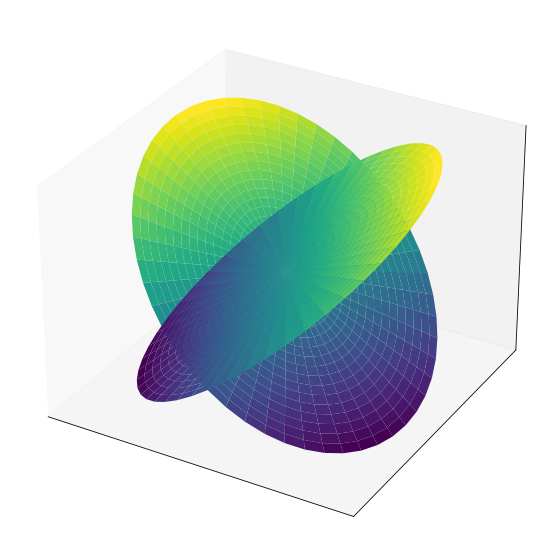
\includegraphics[scale=.35]{doble_disco}
%  \caption{A three dimensional representation of a polydisk in $\mathbb{C}^2$.}
%  \label{fig:polidisco}
%\end{figure}
 
\begin{myprop}{}{pesudo_homo}
The basin of attraction $\mathcal{B}$ of a homogeneous map $F$ is non-empty, pseudoconvex and a complete circular domain. Moreover, $\mathcal{B}$ is bounded if and only if $F$ is non-degenerate.
\end{myprop}

\begin{proof}
Let $r>0$ be a number such that $\|F(Z)\| <1/2 \|Z\|$ if $\|Z\|<r$, given by Lemma \ref{lm:levant02}. Then $B_r = \{Z\in \mathbb{C}^{n+1} \, : \, \|Z\|<r\} \subset \mathcal{B}$, this and the continuity of $F$ implies that $\mathcal{B}$ is an open set. Now notice that if $F^m(Z) \rightarrow 0$, then eventually 
$ F^k(Z) \in B_r$ for $k\geq N$ and some $N>0$. This means that
$$\mathcal{B} = \cup_{k\geq 1} (F^{k})^{-1}(B_r).$$ 
Let $B_n = \{Z\in \mathbb{C}^{n+1} \, : \, \|Z\|<n\}$. Since every euclidean ball is a domain of holomorphy by Theorem \ref{th:geoconvex}, we deduce that each set
$$B_n \cap (F^k)^{-1}(B_r),$$
is a domain of holomorphy by Theorem \ref{th:teohormander} and so pseudoconvex. Then, by Theorem \ref{th:increasingpseudoconvex} we obtain that $(F^{k})^{-1}(B_r)$ is pseudoconvex. Once again, $\{(F^{k})^{-1}(B_r)\}_{k\geq 1}$ is an increasing sequence of pseudoconvex sets so $\mathcal{B}$ is necessarily pseudoconvex.\\

Since $F$ is a homogeneous map of degree $d$, then
$$\|F^j(\alpha Z)\| = |\alpha|^{d^j} \|F^j(Z)\| \leq \|F^j(Z)\|,$$
whenever $|\alpha| \leq 1$, and so it follows that $\mathcal{B}$ is a complete circular domain.\\

Finally, if $F$ is non-degenerate, by Lemma \ref{lm:levant02} it follows that $\mathcal{B} \subset B_R$, where $R>0$ satisfies that $\|F(Z)\| \geq 2 \|Z\|$ whenever $\|Z\|>R$, so $\mathcal{B}$ is bounded. Conversely, if $F$ is degenerate there must be a vector $0\neq Y\in \mathbb{C}^{n+1}$ such that $F(Y)=0$, by homogeneity $F(cY)=0$ for any constant $c\in \mathbb{C}$, so $\mathcal{B}$ is unbounded.
\end{proof}

%\begin{mytheo}
%There exists a unique function $h: \mathbb{C} \rightarrow \mathbb{R}\cup \{-\infty\}$ with the following properties:
%\begin{enumerate}
%\item The function $\alpha(Z) = h(Z)- \log\|Z\|$ is homogeneous of degree $0$, i.e. $\alpha(cZ)=\alpha(Z)$ for all $Z\in \mathbb{C}^{n+1}\setminus \{0\}, c\in \mathbb{C}^*$.
%\item $\mathcal{B} = \{Z \in \mathbb{C}^{n+1} \,:\, h(Z) < 0\}.$
%\end{enumerate}
%\end{mytheo} 
%
%\begin{proof}
%Let $Z\in \mathbb{C}^n\setminus\{0\}$. Define 
%$$\rho(Z) = \sup\{a>0 \,:\, aZ\in \mathcal{B} \}.$$ 
%
%Since $\mathcal{B}$ is completely regular $cZ\in \mathcal{B}$ if and only if $|c|Z\in \mathcal{B}$, whence if $c\in \mathbb{C}^*$
%$$\sup\{a>0 \,:\, a(cZ)\in \mathcal{B} \} = \sup\{a>0 \,:\, (a|c|) Z\in \mathcal{B} \} = \sup\{a/|c|>0 \,:\, a Z\in \mathcal{B} \},$$
%from which it follows that
%$$ \rho(cZ) = \rho(Z)/|c|.$$
%
%Now define $h(Z) = -\log(\rho(Z))$, from the previous paragraph we have $h(cZ) = h(Z) +\log(|c|)$, and so $\alpha(Z) = h(Z) - \log\|Z\|$ is a homogeneous map of degree $0$.\\
%
%Finally, if $Z\in \mathcal{B}$ then $\rho(Z)\geq 1$, and if $Z\not \in \mathcal{B}$ then $\rho(Z)<1$. However, since the iterations of every point in $\mathcal{B}$ eventually belong to an open ball centered at the origin, by continuity of $F$ we get that $\mathbb{B}$ is an open set, from which we must have that $Z\in \mathcal{B}$ if and only if $\rho(Z)>1$, and so $\rho(Z) =1$ if and only if $z\in \partial\mathcal{B}$.  Now it readily follows that
%$$\mathcal{B} = \{Z\in \mathbb{C}^{n+1}\,:\, h(Z) < 0\},$$
%notice that if $cZ\in \mathcal{B}$ for any $c\in \mathbb{C}^*$ then $h(Z) = -\infty$, for example $h(0) = -\infty$. 
%\end{proof}

\begin{mytheo}{}{existence_green}
Let $F:\mathbb{C}^{n+1} \rightarrow \mathbb{C}^{n+1}$ be a homogeneous map of degree $d\geq 2$, then $d^{-j}\log\|F^j(Z)\|$ converges to a plurisubharmonic function $G^F(Z)$ as $j \rightarrow \infty$. The limit $G^F(Z)$ is continuous on $\mathbb{C}^2\setminus\{0\}$ and satisfies the equation
\begin{equation}\label{equation_green}
G^F(F(Z)) = dG^F(Z).
\end{equation} 
If we define $\alpha(Z) \coloneqq G^F(Z)- \log\|Z\|$, then $\alpha$ is a homogeneous map of degree $0$ on $\mathbb{C}^{n+1}\setminus\{0\}$.
\end{mytheo}

\begin{proof}
First suppose $F$ is non-degenerate. Define $\gamma(Z) \coloneqq \log\|F(Z)\| - d \log\|Z\|$, then by Lemma \ref{lm:levant01} there exist $M,m>0$ such that
\begin{equation}\label{equx01}
\log(m) \leq \gamma(Z) \leq \log(M), \qquad \forall\,z\in \mathbb{C}^{n+1}\setminus\{0\},
\end{equation}
so $\gamma$ is bounded. By definition we also have
$$d^{-1}\log\|F(Z)\| = \log\|Z\| + d^{-1}\gamma(Z),$$
evaluating the previous equality at $F^{k-1}(Z)$ and after multiplying both sides by $d^{-k+1}$, we obtain
$$d^{-k}\log\|F^k(Z)\| = d^{-k+1}\log\|F^{k-1}(Z)\| + d^{-k}\gamma(F^{k-1}(Z)).$$
Whence,
\begin{align}\label{equx02}
d^{-j}\log\|F^j(Z)\| &=  d^{-j+1}\log\|F^{j-1}(Z)\| + d^{-j}\gamma(F^{j-1}(Z)) \nonumber\\
&= d^{-j+2}\log\|F^{j-2}(Z)\| + d^{-j+1}\gamma(F^{j-2}(Z)) + d^{-j}\gamma(F^{j-1}(Z)) \nonumber\\
&\vdots \nonumber\\
&= \log( \|Z\|) + d^{-1}\gamma(Z) + \cdots + d^{-j}\gamma(F^{j-1}(Z)).
\end{align}
By equation \eqref{equx01}, if $c=\max\{|\log(m)|,|\log(M)|\}$ we get
$$ \lim_{j \rightarrow \infty} |d^{-1}\gamma(Z)| + \cdots + |d^{-j}\gamma(F^{j-1}(Z))| \leq c \sum_{j\geq 1} \frac{1}{d^j},$$
so $d^{-1}\gamma(Z) + \cdots + d^{-j}\gamma(F^{j-1}(Z))$ converges uniformly on $\mathbb{C}^{n+1}\setminus \{0\}$. Using \eqref{equx02} we deduce that the limit
$$G^F(Z) = \lim_{j\rightarrow \infty}d^{-j}\log\|F^j(Z)\|,$$
exists for all $Z\in \mathbb{C}^{n+1}\setminus\{0\}$. Setting $G^F(0) = -\infty$ we get that $G^F$ is a plurisubharmonic function on $\mathbb{C}^{n+1}$ and continuous at every $Z\neq 0$ by Proposition \ref{pr:convergenceplurisub}. This proves the existence of the limit function $G^F$ when $F$ is non-degenerate.\\

Now, each function $d^{-j}\log\|F^j(Z)\|-\log(\|Z\|)$ is homogeneous of degree $0$ so the same must be true for the limit $\alpha(Z) = G^F(Z)- \log\|Z\|$, and finally
$$\G (F(Z)) = \lim_{j\rightarrow \infty}d^{-j}\log\|F^{j+1}(Z)\| = d\lim_{j\rightarrow \infty}d^{-j-1}\log\|F^{j+1}(Z)\|=d\G(Z),$$
proves \eqref{equation_green}.\\

Suppose now that $F$ is degenerate. For $Z\in \mathbb{C}^{n+1}\setminus\{0\}$ let $h_0(Z) = \log\|Z\| + A$ for $A>0$ large enough such that $\log(M) + (1-d)A<0$. Then,
$$\gamma(Z) \coloneqq h_0(F(Z))-dh_0(Z) \leq \log(M)+(1-d)A<0.$$
Also, it is easy to see that the following relation holds
$$d^{-k}h_0(F^k(Z)) =d^{1-k}h_0(F^{k-1}(Z))+ d^{-k}\gamma(F^{k-1}(Z)).$$
But since $\gamma$ is negative it follows that $\{d^{-k}h_0(F^k)\}$ is a decreasing sequence of plurisubharmonic functions so they converge to a plurisubharmonic function $G^F$ by Proposition \ref{pr:decreasingpluri}. Although this method does also work when $F$ is non-degenerate, we can only assure pointwise convergence. To show the rest of properties for $G^F$ requires no new arguments than in the previous case.
\end{proof}

\begin{mydef}{}{def_green}
The function $G^F$ given in Theorem \ref{th:existence_green} is called the (dynamical) {\bf Green function} of $F$.\nomenclature[20]{$\G$}{Dynamical Green function associated to $F$}
\end{mydef}

\begin{mytheo}{}{}
Let $F:\mathbb{C}^{n+1} \rightarrow \mathbb{C}^{n+1}$ be a homogeneous map of degree $d\geq 2$, then
$$\mathcal{B} = \{Z \in \mathbb{C}^{n+1} \,:\, \G (Z) < 0\}.$$
\end{mytheo}

\begin{proof}
Suppose that $F^j(Z) \rightarrow 0$ then $d^{-j}\log (\|F^j(Z)\|)<0$ eventually, so $G^F(Z)\leq 0$ for all $Z\in \mathcal{B}$. On the other hand, by equation \eqref{equation_green} we get
$$\G (F^j(Z)) = d^j \G(Z),$$
so if $G^F(Z)>0$ then $Z\not \in \mathcal{B}$. Now, by continuity of $\G$ on $\mathbb{C}^{n+1}$ the set $(G^F)^{-1}(-\infty,0]$ must be a proper closed subset, but $\mathcal{B}$ is open, so $\G (Z)<0$ if and only if $Z\in \mathcal{B}$.
\end{proof}

\begin{myprop}{}{}
If $F:\mathbb{C}^{n+1} \rightarrow \mathbb{C}^{n+1}$ is a non-degenerate homogeneous map of degree $d\geq 2$, then the associated dynamical Green function $G^F$ satisfies
\begin{equation}\label{equgreen01}
G^F(c\cdot Z) = G^F(Z) + \log|c|,
\end{equation}
and
\begin{equation}\label{equgreen02}
G^{c\cdot F}(Z) = G^F(Z) + \frac{1}{d-1}\log|c|,
\end{equation}
for any $Z\in \mathbb{C}^{n+1}$ and $c\in \mathbb{C}^*$.
\end{myprop}

\begin{proof}
We have
\begin{align*}
G^F(c\cdot Z) &= \lim_{j\rightarrow \infty} \frac{1}{d^j} \log\| F^j(cZ)\| \\
&=  \lim_{j\rightarrow \infty} \frac{1}{d^j} \log\| c^{d^j}F^j(Z)\|\\
&= \lim_{j\rightarrow \infty} \frac{1}{d^j}\log\|F^j(Z)\| + \log|c|\\
&= G^F(Z) + \log|c|,
\end{align*}
which proves the first identity. Similarly,
\begin{align*}
G^{c\cdot F}(Z) &= \lim_{j\rightarrow \infty} \frac{1}{d^j} \log\| (cF)^j(Z)\| \\
&= \lim_{j\rightarrow \infty} \frac{1}{d^j} \log\| c^{1+d+\cdots+d^{j-1}}\cdot F^j(Z)\| \\
&= G^F(Z) + \lim_{j\rightarrow \infty} \log|c|(\sum_{k=1}^{j} d^{-k})\\
&= G^F(Z) + \log|c|\frac{d}{d-1},
\end{align*}
from which the second identity follows and we are done.
\end{proof}

\section{Measure of maximal entropy}\label{sectionmaximummeasure}

The approach and proofs of this section are based in \cite{lopes}. Let $f:\mathbb{P}^1 \rightarrow \mathbb{P}^1$ be a rational function, denote by $\{z_i^n(a)\}_{i=1}^{d^n}$ the roots of the equation $f^n(z)=a$, counted with multiplicity. In this section we show that the measures
\begin{equation}\label{diracs}
\mu_n\coloneqq \frac{1}{d^n}\sum_{i=1}^{d^n} \delta_{z_i^n(a)},
\end{equation}
where $\delta_x(y)=1$ only for $y=x$ and otherwise $\delta_x(y)=0$, are weak$^*$-convergent to a measure $\mu_f$, called {\bf measure of maximum entropy},\nomenclature[21]{$\mu_f$}{Measure of maximum entropy for $f$} which is independent of $a$, as long as $a$ is a non-exceptional point. The \emph{push-forward measure} of a probability measure $\mu$ by $f$ is defined by $f_*\mu(E) = \frac{1}{d}\mu \circ f^{-1}(E)$, for all measurable subsets $E$, where $d$ is the degree of $f$. Then we can see that $\mu_n = (f^n)_*\delta_a$, so $\mu_n$ is the push-forward by $f^n$ of $\delta_a$.\\

In the following, $f:\mathbb{P}^1 \rightarrow \mathbb{P}^1$ will always denote a rational function.\\

\begin{mydef}{}{defadapted}
A set $U\subset \mathbb{P}^1$ is said to be {\bf $(N,\varepsilon)$-adapted} if for all $n\geq N$ there exist topological disks $S_i^n$, and integers $1\leq k_i(n)$ for $i=1,\dots,l_n$ such that 
\begin{enumerate}
\item $f^n|_{S_i^n}$ is a $k_i(n)$-to-$1$ map onto $U$.\\
\item $\diam(S_i^n) \leq \varepsilon$.\\
\item $\sum_{i=1}^{l_n}k_i(n) \geq (1-\varepsilon)d^n$.\\
\item $\lim_{n \rightarrow +\infty} (\sup_{i} \diam (S_i^n))=0.$
\end{enumerate} 
\end{mydef}

Some drawings may be useful to grasp what is required in Definition \ref{df:defadapted}. In Figure \ref{fig:adaptedfig} the topological disks $S^n_i$ are represented; whereas in Figure \ref{fig:adaptedfig2} is a representation of how $f^n$ acts on a particular $S_i^n$, in this example the region is subdivided into $k_i(n)$ subsets on which $f^n$ is bijective, a circle of radius $\varepsilon$ contains $S_i^n$ so $\diam(S_i^n)\leq \varepsilon$. Condition $3$ in Definition \ref{df:defadapted} gives an upper bound on how many preimages under $f^n$ of each point in $U$ the set $\cup_{i=1}^{k_i(n)} S_i^n$ may fail to contain, specifically $\lfloor \varepsilon d^n \rfloor$, where $\lfloor x \rfloor$ denotes the greatest integer $n$ such that $n\leq x$. Condition $4$ simply states that the diameters of the topological disks $S_i^n$ tend uniformly to $0$.

\begin{figure}[h!]
	\centering  
  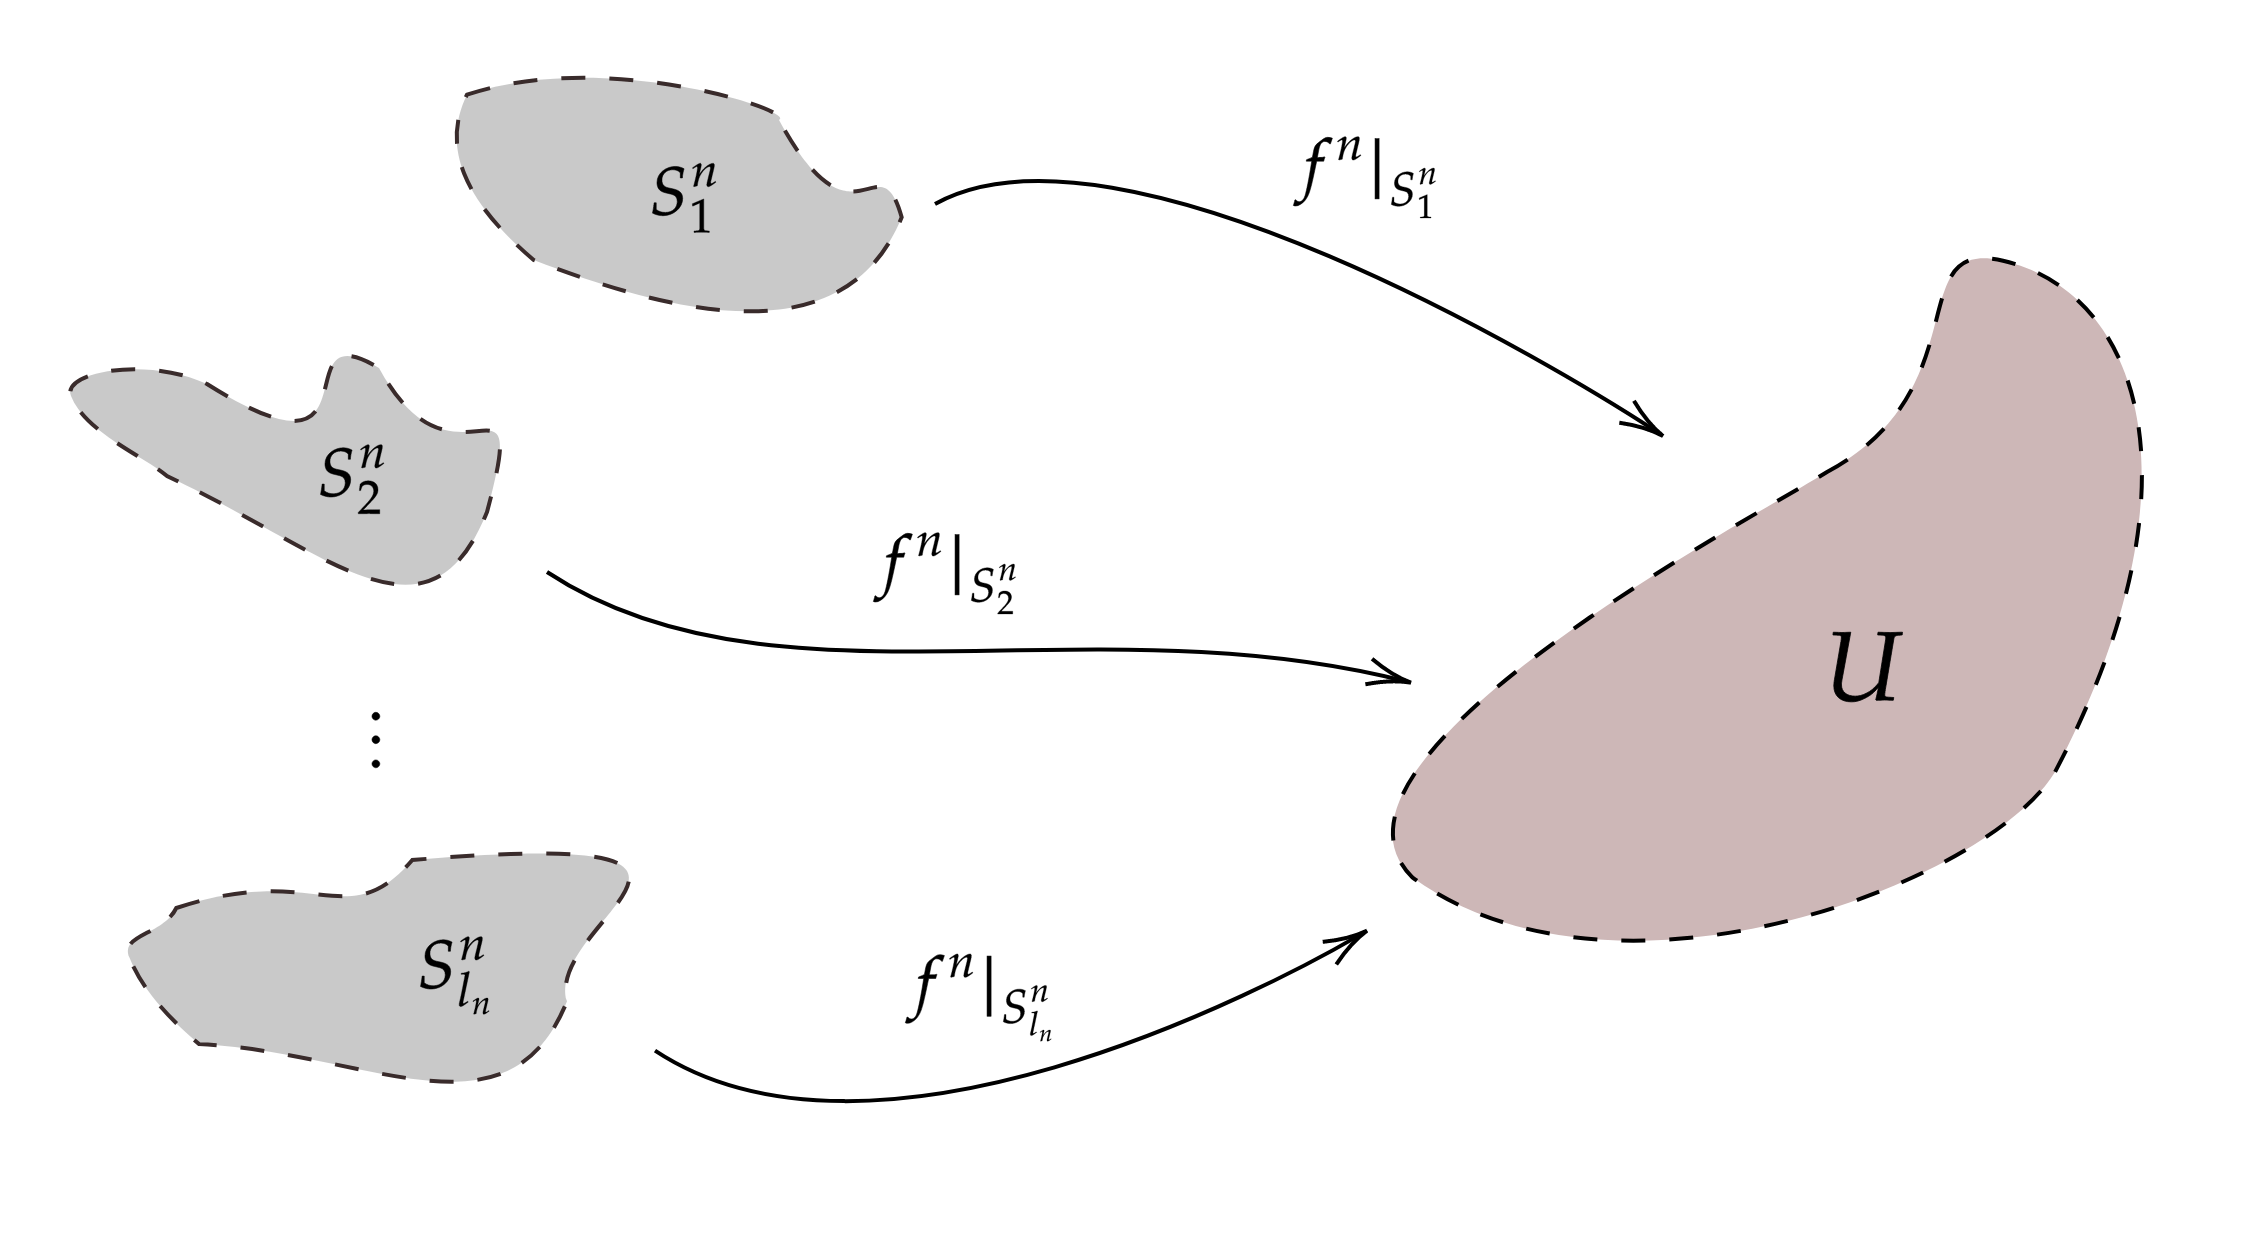
\includegraphics[scale=.19]{d003}
  \caption{Each topological disk $S_i^n$ is mapped under $f^n$ onto $U$.}
  \label{fig:adaptedfig}
\end{figure}

\begin{figure}[h!]
	\centering  
  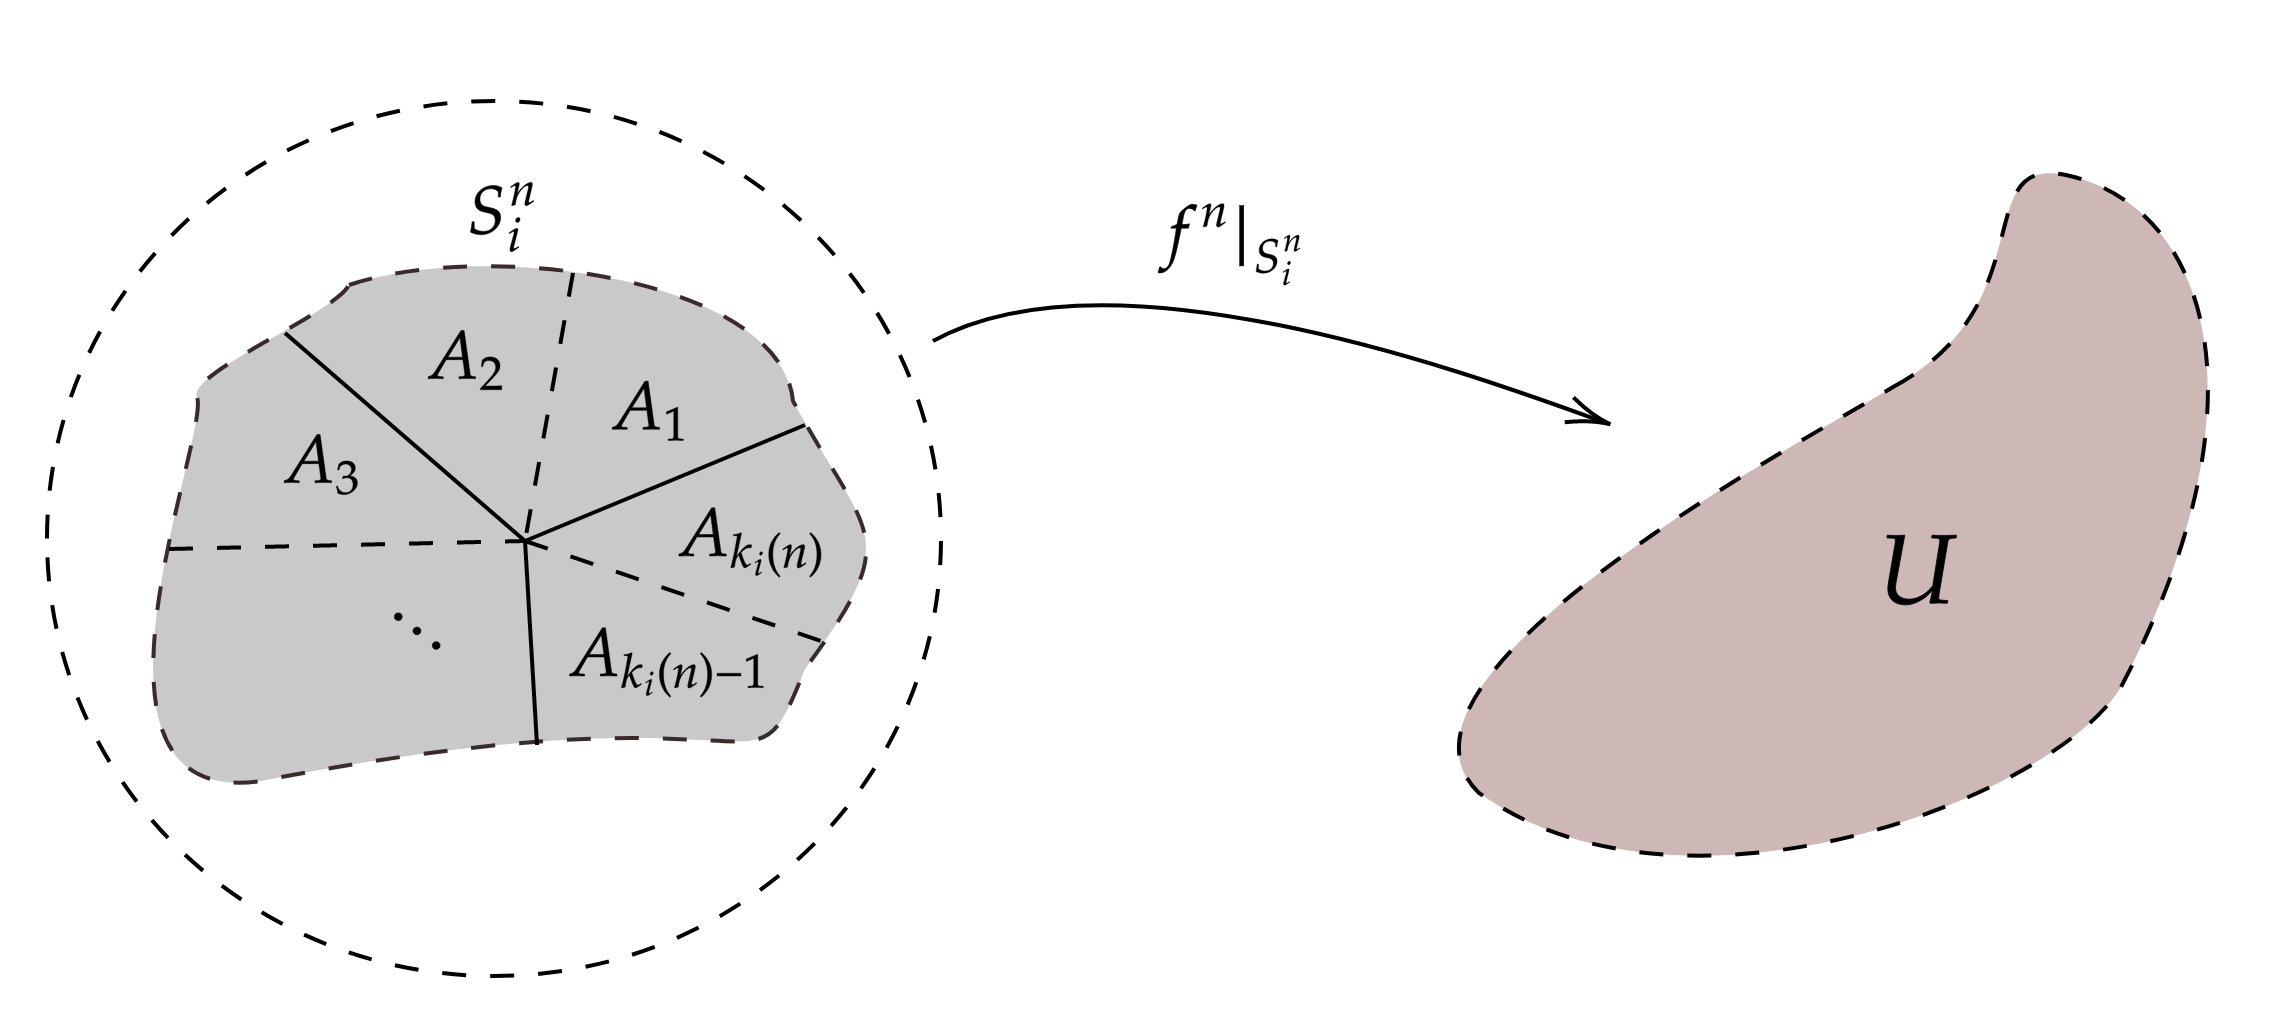
\includegraphics[scale=.18]{d005}
  \caption{Each region $A_i$ is mapped bijectively by $f^n$ onto $U$.}
  \label{fig:adaptedfig2}
\end{figure}

\begin{myexmp}[breakable]{}{}
Consider $p(z)=z^2$ and $U=\{re^{i\theta}\,:\, 2<r<3, 0<\theta<1\}$. We will show that given $\varepsilon>0$ the set $U$ is $(N,\varepsilon)$-related for sufficiently large $N$.\\
First, notice that
\begin{align*}
p^{-1}(U) &= \{re^{i\theta}\,:\, 2^{1/2}<r<3^{1/2}, 0<\theta<1/2\}\\
&\cup \{re^{i(\theta+\pi)}\,:\, 2^{1/2}<r<3^{1/2}, 0<\theta<1/2\}.
\end{align*}
Upon this observation it is not difficult to see that for every $n\geq 1$ the set $p^{-n}(U)$ can be expressed as union of $2^n$ disjoint sets of the form $\{re^{i\theta}\,:\, 2^{1/2^n}<r<3^{1/2^n}, a<\theta<b\}$ where $|b-a| \mod 2\pi < 1/2^n$, these sets are actually the connected components of $p^{-n}(U)$. Hence, let $\{S_i^n\}_{i=1}^{2^n}$ be the connected components of $p^{-n}(U)$, numbered in any manner. Also let $l_n=2^n$. It is readily seen that $\lim_{n\rightarrow \infty} \sup_i \diam (S_i^n)=0$, in fact for a given $n$ all the $S_i^n$ have the same diameter. The map $f^n|_{S_i^n}$ is bijective, so let $k_i(n)=1$ for $i=1,\dots,2^n$. It follows that $\sum_{i=1}^{2^n}k_i(n)>(1-\varepsilon)d^n$ for every $n\geq 1$. Finally, let $N>0$ be the least integer such that $\diam(S_i^m) \leq \varepsilon$ for some $i$. From what has been discussed it follows that $U$ is $(N,\varepsilon)$-related.
\end{myexmp}

\begin{mydef}{}{}
Two points $z_i\in \mathbb{P}^1$, $i=1,2$, are {\bf $(N,\varepsilon)$-related} if for all $n\geq N$ the roots $z_i^n(z_1)$ of the equation $f^n(z) = z_1$ and the roots $z_i^n(z_2)$ of the equation $f^n(z) = z_2$ can be indexed such that
$$d(z_i^n(z_1),z_i^n(z_2)) \leq \varepsilon,$$
holds for every $i=1,\dots,t_n$, where $t_n\geq 1$ satisfies $t_n \geq (1-\varepsilon)d^n$.
\end{mydef}

\begin{myexmp}[breakable]{}{}
Consider again $p(z)=z^2$. Let $z_1=re^{i\theta}$ for some $r>0$ and $0<\theta<2\pi$. Take a number $0<\eta<2\pi$ such that $\eta-\theta \mod 2\pi \neq 0$ and define $z_2= re^{i(\theta+\eta)}$. We will show that given $\varepsilon>0$ the points $z_1$ and $z_2$ are $(N,\varepsilon)$-related for sufficiently large $N$.

For each $n\geq 1$, let $\{z_i^n(z_1)\}_{i=1}^{2^n}$ be the roots of the equation $p^n(z)=z_1$. Let $z_i^n(z_2) = z_i^n(z_1)\cdot e^{i\eta/2^n}$ for $i=1,\dots,2^n$. It follows that $p^{-n}(z_2) = \{z_i^n(z_2)\}_{i=1}^{2^n}$. Moreover, $|z_i^n(z_1)-z_i^n(z_2)|<\eta/2^n$ for each $i=1,\dots,2^n$. Let $t_n=2^n$ for every $n\geq 1$. Take the least integer $N>0$ such that $\eta/2^N\leq \varepsilon$. It follows that the points $z_1,z_2$ are $(N,\varepsilon)$-related.   
\end{myexmp}

\begin{myprop}{}{prop-adapted}
If $z_i$ belongs to an $(N,\varepsilon)$-adapted set $U_i$, $i=1,2$, and $U_1\cap U_2 \neq \emptyset$, then $z_1,z_2$ are $(N,2\varepsilon)$-related. 
\end{myprop}

\begin{proof}
Take $z_0 \in U_1\cap U_2$ and let $n\geq N$, then there exists an integer $t_{1n}\geq (1-\varepsilon)d^n$ ($t_{1n}$ equals the sum $\sum k_i(n)$ given in the definition of $(N,\varepsilon)$-adapted set for $U_1$) such that $(f^{n})^{-1}(z_1)$ and $(f^n)^{-1}(z_0)$ can be numbered in such a way that
$$d(z_i^n(z_0),z_i^n(z_1)) \leq \varepsilon \quad i=1,\dots,t_{1n},$$
where $(f^{n})^{-1}(z_j) = \{z_i^n(z_j)\}_{i=1}^{d^n}$, $j=1,2$. Using that $U_2$ is $(N,\varepsilon)$-adapted, then we can also numerate the sets $(f^{n})^{-1}(z_1)$ and $(f^n)^{-1}(z_0)$ in such a manner that
$$d(z_{2i}^n(z_0),z_i^n(z_2)) \leq \varepsilon \quad i=1,\dots,t_{2n},$$
where $(f^{n})^{-1}(z_2) = \{z_i^n(z_2)\}_{i=1}^{d^n}$, $(f^{n})^{-1}(z_0) = \{z_{2i}^n(z_0)\}_{i=1}^{d^n}$ and $t_{2n}\geq (1-\varepsilon)d^n$. Taking $t_n = \min\{t_{1n},t_{2n}\}$ we can suppose that the order of the first $t_n$ terms in $(f^n)^{-1}(z_0)$ is the same in the two previous cases so that
$$d(z_i^n(z_1),z_i^n(z_2)) \leq 2\varepsilon \quad i=1,\dots,t_{n},$$
proving that $z_1,z_2$ are $(N,2\varepsilon)$-related. 
\end{proof}

The existence of the measure $\mu_f$ will be derived from the next lemma, whose proof can be found in $\cite{lopes}$. Recall from Definition \ref{df:def_exceptional} that $\Exc(f)$ denotes the set of exceptional points of $f$.

\begin{mylema}{Fundamental Lemma}{fund}
Let $\varepsilon>0$, $z\not \in \Exc(f)$ and an arc $\gamma$ containing $z$ and such that $\gamma\setminus \{z\}$ does not contain critical values of $f^n$ for all $n\geq 1$, then there exists an $(N,\varepsilon)$-adapted set $U\supset \{\gamma\}$ for some $N\geq 1$.
\end{mylema}

\begin{mycoro}{}{equ-makesense}
Let $\varepsilon>0$. If $z_1,z_2\not \in \Exc(f)$ then there exists an open set $V\supset\{z_1,z_2\}$ such that any couple of points in $V$ is $(N,\varepsilon)$-related for some $N>0$.
\end{mycoro}

\begin{proof}
Construct arcs $\gamma_i\supset \{z_i\}$ such that they do not contain critical values of $f^n$ for all $n\geq 1$ aside from, maybe, $\{z_i\}$ and such that $\gamma_1\cap \gamma_2\neq \emptyset$. Then by the Fundamental Lemma \ref{lm:fund} there exist $(N_i,\varepsilon/2)$-adapted sets $U_i \supset \gamma_i$, $i=1,2$. Then $U_1,U_2$ are $(N,\varepsilon/2)$-adapted sets, with $N=\max\{N_1,N_2\}$. Since $U_1\cap U_2\neq \emptyset$ then by Proposition \ref{pr:prop-adapted} any two points in $U_1\cup U_2$ are $(N,\varepsilon)$-related.
\end{proof}

\begin{mycoro}{}{coro2}
Given a compact set $K\subset \mathbb{P}^1\setminus \Exc(f)$ and $\varepsilon>0$ there exists $N = N(K,\varepsilon)$ such that any couple of points in $K$ is $(N,\varepsilon)$-related.
\end{mycoro}

\begin{proof}
Define $M:K\times K \rightarrow \mathbb{N}$ by setting $M(z_1,z_2)$ as the minimum $N>0$ such that there exist neighborhoods $V_i$ of $z_i$, $i=1,2$, such that every point in $V_1$ is $(M(z_1,z_2),\varepsilon)$-related to every point in $V_2$. Notice that from Corollary \eqref{cr:equ-makesense} the previous minimum actually exists and so $M$ is a well defined function. Moreover, by definition if $(z_1,z_2)\in V_1\times V_2$, where every point in $V_1$ is $(N(z_1,z_2),\varepsilon)$-related to every point in $V_2$, then taking the same neighborhoods it follows that for any $(z_3,z_4)\in V_1\times V_2$ one must have $M(z_3,z_4) \leq M(z_1,z_2)$ from which we get
$$\limsup_{(z_3,z_4) \rightarrow (z_1,z_2)}M(z_3,z_4) \leq M(z_1,z_2),$$
showing that $M(\cdot,\cdot)$ is an upper semicontinuous function. Since every upper semicontinuous function is bounded above on compact sets, $M$ is bounded on $K\times K$, if $N>0$ is an upper bound for $M$ on $K\times K$ every pair of points in $K$ is $(N,\varepsilon)$-related.
\end{proof}

\begin{mycoro}{}{coro3}
If $K\cap \Exc(f)=\emptyset$ and $K$ is compact, then for all $\varepsilon_1>0$ and every continuous function $\phi:\mathbb{P}^1\rightarrow \mathbb{R}$, there exists $N(K,\varepsilon_1,\phi)$ such that
$$\left| \int_{\mathbb{P}^1}\phi \, d\mu_n(z_1)-\int_{\mathbb{P}^1} \phi\, d\mu_n(z_2) \right| \leq \varepsilon_1,$$
for every $z_1$ and $z_2$ in $K$ and $n\geq N$.
\end{mycoro}

\begin{proof}
Let $\phi:\mathbb{P}^1\rightarrow \mathbb{R}$ be a continuous function. Since $\mathbb{P}^1$ is compact, we can take $\varepsilon>0$ satisfying
$$\varepsilon \sup_{z\in \mathbb{P}^1}|\phi(z)| \leq \varepsilon_1/4,$$
and since $\phi$ is uniformly continuous we can suppose that $\varepsilon$ is small enough such that $d(z,z')<\varepsilon$ implies $|\phi(z)-\phi(z')| \leq \varepsilon_1/2$. Now define $N(K,\varepsilon_1,\phi)$ as the integer given by Corollary \ref{cr:coro2} applied to $K$ and $\varepsilon$. Then any pair of points in $K$ is $(N,\varepsilon)$-related, so if $z_1,z_2\in K$ we can index the roots $z_i^n(z_1)$ of the equation $f^n(z) = z_1$, and the roots $z_i^n(z_2)$ of $f^n(z) = z_2$ in such a manner that $d(z_i^n(z_1),z_i^n(z_2))\leq \varepsilon$ for $i=1,\dots, s_n$, where $s_n$ satisfies $s_n \geq (1-\varepsilon)d^n$. So
\begin{align*}
\left| \int_{\mathbb{P}^1}\phi\,d \mu_n(z_1) - \int_{\mathbb{P}^1}\phi\,d \mu_n(z_2) \right| &\leq \frac{1}{d^n} \sum_{i=1}^{d^n} | \phi(z_i^n(z_1))-\phi(z_i^n(z_2)|\\
&=\frac{1}{d^n} \sum_{i=1}^{s^n} | \phi(z_i^n(z_1))-\phi(z_i^n(z_2))|\\
&+ \frac{1}{d^n} \sum_{i=s_n+1}^{d^n} | \phi(z_i^n(z_1))-\phi(z_i^n(z_2))|\\
&\leq  \frac{1}{d^n} \sum_{i=1}^{s_n} \varepsilon_1/2 + 2\,\frac{d^n-s_n}{d^n} \sup_{z\in \mathbb{P}^1}|\phi(z)|\\
& \leq \frac{s_n}{d^n} \, \varepsilon_1/2 +2\, \varepsilon \sup_{z\in \mathbb{P}^1}|\phi(z)| \\
&\leq \varepsilon_1/2 + \varepsilon_1/2 = \varepsilon_1.\\
\end{align*}
\end{proof}

\begin{mylema}{}{suma}
If $m>n\geq 1$ and $k=m-n$ then
$$\int_{\mathbb{P}^1} \phi \, d\mu_m(z) = \frac{1}{d^k} \sum_{i=1}^{d^k} \int_{\mathbb{P}^1} \phi \,d\mu_n(z_i^k(z)).$$
\end{mylema}

\begin{proof}
Notice that
$$\int_{\mathbb{P}^1} \phi \, d\mu_n(z_i^k(z)) = \frac{1}{d^n} \sum_{j=1}^{d^n} \phi (z_j^n(z_i^k(z))),$$
so we have
$$\frac{1}{d^k}\sum_{i=1}^{d^k} \int_{\mathbb{P}^1} \phi \,d\mu_n(z_i^k(z)) = \frac{1}{d^m}\sum_{i=1}^{d^k}\sum_{j=1}^{d^n} \phi (z_j^n(z_i^k(z))),$$
since for $i,j$ we can find an $1\leq l \leq d^m$ satisfying $z_l^m(z) = z_j^n(z_i^k(z))$, we can construct a bijective relation between the roots and get
$$\frac{1}{d^m}\sum_{i=1}^{d^k}\sum_{j=1}^{d^n} \phi (z_j^n(z_i^k(z))) = \frac{1}{d^m} \sum_{j=1}^{d^m} \phi(z_j^m(z)) = \int_{\mathbb{P}^1} \phi \,d\mu_m.$$
\end{proof}

\begin{mycoro}{}{coro4}
Given a compact set $K\cap \Exc(f)=\emptyset$, a number $\varepsilon_1>0$ and a continuous function $\phi:\mathbb{P}^1 \rightarrow \mathbb{R}$, there exists $N>0$ such that 
$$\left | \int_{\mathbb{P}^1} \phi \, d\mu_n(z) - \int_{\mathbb{P}^1}\phi \, d\mu_m(z) \right | \leq \varepsilon_1,$$
for every $z\in K$ and $n,m\geq N$.\\
\end{mycoro}

\begin{proof}
Set $\tilde{K} = \overline{\cup_{n\geq 0} f^{-n}(K)}\subset \mathbb{P}^1$, then $\tilde{K}$ is compact and does not contain exceptional points. To justify the latter, by Theorem \ref{th:exceptional} $f$ is conjugated either to a polynomial $g$ for which $\infty$ is the only exceptional point or to a map of the form $z^d$ where $|d|\geq 2$ is an integer. For the first case it is sufficient to consider a compact set $E\subset D_\infty\setminus \{\infty\}$ where $D_\infty$ is the Fatou component associated to $g$ containing $\infty$: as the points in $g^{-n}(z)$ converge to $\partial D_\infty$ for $z\in D_\infty\setminus \{\infty\}$ it is clear that $g^{-n}(E)$ is contained in the complement of a neighborhood of $\infty$ for every $n\geq 1$ so $\infty\not \in \overline{\cup_{n\geq 1} g^{-n}(E)}$, implying that $\tilde{K}$ does not contain the exceptional point of $f$.\\

In case $f$ in conjugated to $g(z)=z^d$ where $d\geq 2$, then the points in $g^{-n}(z)$ have modulus converging asympotically to $1$. Hence, for any $z\neq 0,\infty$ the set $\cup_{n\geq 1} g^{-n}(z)$ is contained in a neighborhood of $\partial D(0,1)$, which is sufficient to get the desired conclusion.\\

If $f$ is conjugated to some $z^{-d}$ where $d\geq 2$, then $f^{n}$ is conjugated to $h\circ g^n$, where $h(z)=1/z$ and $g(z)=z^d$. Since the points in the set $g^{-n}(h^{-1}(z))$ have modulus converging asymptotically to $1$ for $z\neq 0,\infty$, the desired conclusion is also obtained in this case.\\

Now take $z \in K$, using Lemma \ref{lm:suma} we obtain
\begin{align*}
\left| \int_{\mathbb{P}^1} \phi \, d\mu_n(z) - \int_{\mathbb{P}^1}\phi \, d\mu_m(z) \right | & \leq \frac{1}{d^k} \sum_{i=1}^{d^k} \left |\int_{\mathbb{P}^1} \phi \, d\mu_n(z) - \int_{\mathbb{P}} \phi \,  d\mu_n(z_i^k(z)) \right|
\end{align*}
by construction every $z_i^k(z)$ is contained in $\tilde{K}$ , so if $n\geq N$ where $N$ is given in Corollary \ref{cr:coro3} we can bound from above the last term by $\frac{1}{d^k}d^k\varepsilon_1 = \varepsilon_1$. 
\end{proof}

\begin{mytheo}{}{theo_Lopes}
There exists an $f$-invariant probability measure $\mu_f$ such that
\begin{enumerate}
\item $ \mu_n(a) \overset{w^*}{\to} \mu_f$ when $a\not \in \text{Exc}(f)$, and the convergence is uniform if $a$ varies in a compact subset of $\mathbb{C} \setminus \text{Exc}(f)$.

\item $\supp(\mu_f) = J(f)$.\\
\end{enumerate}
\end{mytheo}

\begin{proof}
Take $z\not \in \Exc(f)$, then by Corollary \ref{cr:coro4} the mapping 
$$\phi \mapsto\lim_{n \rightarrow \infty} \int_{\mathbb{P}^1} \phi\, d\mu_n(z),$$
is well defined and also defines a continuous linear functional on $C(\mathbb{P}^1)$, the space of continuous functions $\phi:\mathbb{P}^1 \rightarrow \mathbb{R}$. So there exists a measure $\mu_f(z)$ such that $\mu_n(z) \overset{w^*}{\rightarrow} \mu_f(z)$, by Corollary \ref{cr:coro3} this measure does not depend on the point $z$ so we can write only $\mu_f$ for the limit. The measure $\mu_f$ is $f$-invariant since for any $a\not \in \Exc(f)$
\begin{align*}
\int_{\mathbb{P}^1} (\phi\circ f) \,d\mu_f &= \lim_{n \rightarrow \infty} \frac{1}{d^n} \sum_{i=1}^{d^n}\phi(f(z_i^n(a))\\
& = \lim_{n \rightarrow \infty} \frac{1}{d^{n-1}} \sum_{i=1}^{d^{n-1}}\phi((z_i^{n-1}(a)) = \int_{\mathbb{P}^1}\phi \,d\mu_f.
\end{align*}

Now we have to prove $\supp(\mu_f)=J(f)$. Firstly take $a\in J(f)$, by complete invariance of the Julia set it follows that $\supp(\mu_n(a)) \subset J(f)$ for every $n\geq 1$, but then it is straightforward that $\supp(\mu_f) \subset J(f)$. Conversely, take $p\in J(f)$ and any $q\in \supp(\mu_f)$, then we know that $q\in J(f)$ and by Theorem \ref{th:exceptional-julia} $J = \overline{O^-(q)}$, so there exists a sequence $p_n \rightarrow p$ and a sequence of integers $m_n \rightarrow +\infty$ such that $f^{m_n}(p_n)=q$. If we show that each $p_n$ belongs to $\supp(\mu_f)$ then it would follow that $p\in \supp(\mu_f)$ because the support of a measure is a closed set. Given any neighborhood $V$ of $p_n$ take a neighborhood $U$ of $p_n$ such that $U\subset V$ and $\mu_f(\partial U)=0$ (if no such $U$ exists, then $p_n$ belongs to $\supp(\mu_f)$ and we are done). Then by the Open Mapping Theorem and $f$-invariance $\mu_f(\partial (f^{m_n}(U)))=0$. Using that these boundaries have measure $0$ we can write
\begin{equation}\label{equu01}
\mu_f(U) = \lim_{n \rightarrow +\infty} \mu_n(a)(U) = \lim_{j \rightarrow \infty} \frac{1}{d^j}\left|\{z\in U\,:\, f^j(z) =a\}\right|,
\end{equation}
and 
\begin{equation}\label{equu02}
\mu_f(f^{m_n}(U)) = \lim_{j \rightarrow+\infty} \mu_j(a)(f^{m_n}(U)) = \lim_{j \rightarrow +\infty}\frac{1}{d^j} \left| \{ z\in f^{m_n}(U) \,:\, f^j(z)=a\}\right|.
\end{equation}

If $a$ is chosen so that it is not an exceptional point and is neither a critical value of any $f^j$, then each root of the equation $f^n(z) = a$ is simple so
$$\left | \{z\in U\,:\, f^j(z) =a\}\right| \geq \left |\{z\in f^{m_n}(U) \,:\,f^{j-m_n}(z)=a\}\right|,$$
but then
$$\frac{1}{d^j}\left| \{z\in U\,:\, f^j(z) =a\}\right| \geq \frac{1}{d^{j}}\left| \{z\in f^{m_n}(U) \,:\,f^{j-m_n}(z)=a\} \right|.$$
This together with \eqref{equu01} and \eqref{equu02} imply
\begin{align*}
\mu_f(V)&\geq \mu_f(U)\\ &\geq \frac{1}{d^{m_n}}\lim_{j\rightarrow \infty} \frac{1}{d^{j-m_n}}\left| \{z\in f^{m_n}(U) \,:\,f^{j-m_n}(z)=a\} \right|\\
&\geq \frac{1}{d^{m_n}}\mu_f(f^{m_n}(U))>0,
\end{align*}
where $\mu_f(f^{m_n}(U))>0$ because $f^{m_n}(U)$ is a neighborhood of $q$. 
\end{proof}

\begin{myrmk}{}{}
A stronger result states that actually $(f^n)_*(\mu)$ converges to $\mu_f$ whenever the measure $\mu$ satisfies $\mu(\Exc(f))=0$, see \cite[Theorem 4.1(a)]{hubbard}. 
\end{myrmk}

\begin{myrmk}{}{}
Let $f$ be a rational function of degree $d\geq 2$ over $\C$. Let $h(f)$ be the topological entropy of $f$ and $h_\mu(f)$ the measure theoretic entropy of $f$ with respect to an $f$-invariant measure $\mu$, see \cite[Chapter 11]{hawkins} for definitions. The Variational Principle of Entropy \cite[Theorem 11.40]{hawkins} states that 
$$h(f) = \sup\{h_\mu(f) \,:\, \mu \text{ is an $f$-invariant Borel probability measure}\}.$$
It can be shown that $h(f) = \log d$ and that $h_{\mu_f}(f) = \log d$, see \cite[Theorem 8.3.1]{katok} and \cite{gromov}. Therefore, $\mu_f$ is called measure of maximal entropy.
\end{myrmk}

\begin{myexmp}{}{exracionales}
Consider $f(z) = z^2$, take $a\in \mathbb{C}^*$. Then, for each $n\geq 1$, the set $f^{-n}(a)$ is composed by $2^n$ points uniformly distributed in a circle of radius $|a|^{1/2^n}$, see Figure \ref{fig:raices}. Since $\lim_{n\rightarrow \infty} |a|^{1/n}=1$ it follows that these roots accumulate about $J(f)$ uniformly. In particular, when $|a|=1$, the sequence of measures 
$$\mu_n = \frac{1}{d^n}\sum_{i=1}^{d^n} \delta_{z_i^n(a)},$$
converges {\it set-wise} to the normalized arc length measure $\lambda$ on $\mathbb{S}^1 = \{|z|=1\}$, that is,
$$\lim_{n\rightarrow \infty} \mu_n(E) = \lambda(E),$$
for any Borel subset $E\subset J(f)$. It can be shown that set-wise convergence implies wea$\text{k}^*$-convergence, see \cite[Corollary 4.7.26]{bogachev}. The same conclusion can be reached evidently for any polynomial of the form $f(z) = z^n$ where $n\geq 2$.\\

Consider now $f(z)=z^{-2}$ and for simplicity assume that $|a|=1$. Notice that $f^n(z) = z^{(-1)^n2^n}$, so the roots of the equation $f^n(z)-a=0$ are either the roots of the equation $(z^2)^n -a=0$ or the roots of $(z^2)^n -\bar{a}=0$. In both cases, the roots are uniformly distributed along $\mathbb{S}^1$. This implies again that $\mu_f$ is the normalized arc length measure on $\mathbb{S}^1$. As before, a similar argument holds for any function given by $f(z) = z^n$ where $n\leq -2$.\\

In conclusion if $\mu_f$ is a polynomial of the form $z^n$ with $|n|\geq 2$, then $\mu_f$ is the normalized arc length measure on $\mathbb{S}^1$.
\end{myexmp}

\begin{figure}[h!]
	\centering  
  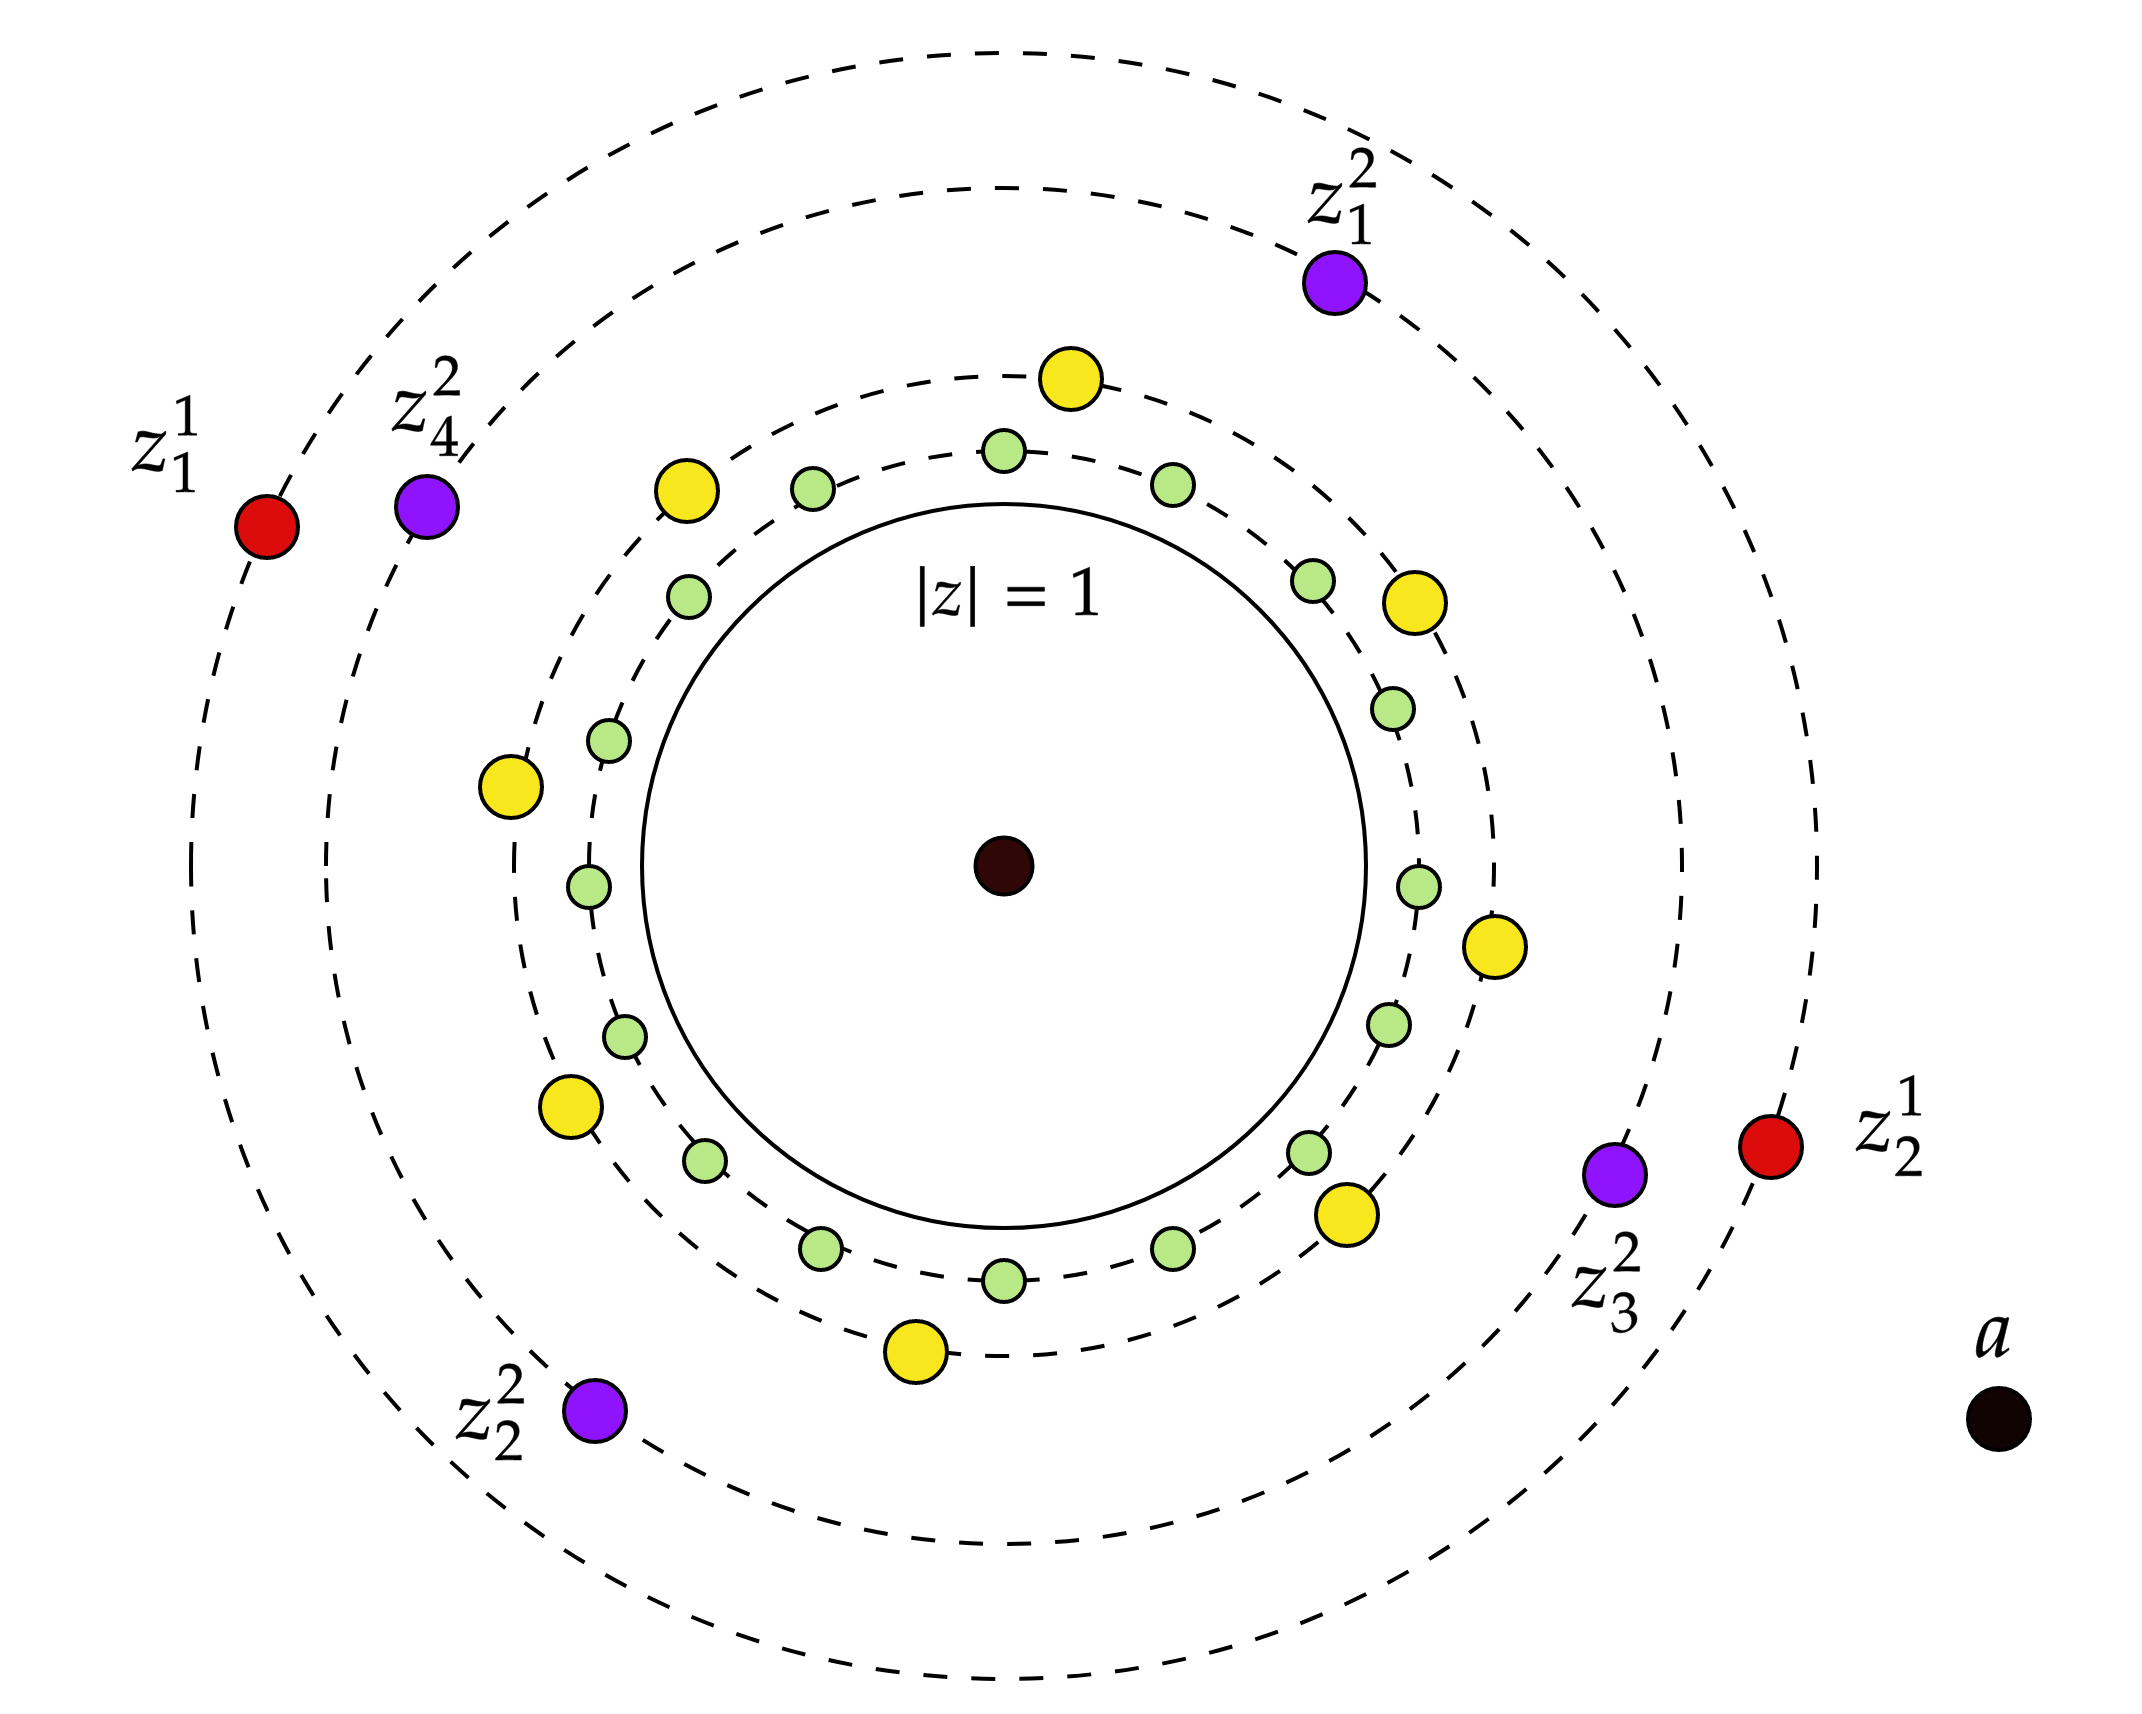
\includegraphics[scale=.16]{raices}
  \caption{Distribution of the roots of $z^{2n}-a =0$ for a point $|a|>1$ and $n=1,2,3,4$.}
  \label{fig:raices}
\end{figure}

\section{Weighted potential theory}\label{seccionweighted}

Let $f$ be a rational function on $\mathbb{P}^1$ of degree $1$ and let $F(z_0,z_1) = (F_0(z_0,z_1),F_1(z_0,z_1))$ be a lift of $f$ (see Section \ref{sec:secciongreen} and Appendix \ref{p1}). We define a  product $\wedge \colon \mathbb{C}^2\times \mathbb{C}^2 \rightarrow \mathbb{C}$ by $(z_0,z_1)\wedge(w_0,w_1) \coloneqq z_0 w_1 - z_1 w_0$. Under this definition it is a straightforward calculation to check that $(cZ)\wedge W = Z\wedge(cW) = c(Z\wedge W)$ for all $Z,W\in \mathbb{C}^2$ and $c\in \mathbb{C}^*$.\\
Now define the weighted kernel $\Phi_F: \mathbb{P}^1 \times \mathbb{P}^1 \rightarrow \mathbb{R}\cup\{-\infty\}$ as
$$\Phi_F(z,w) \coloneqq \log |Z\wedge W| -G^F(Z)-G^F(W) \in \mathbb{R}\cup \{-\infty\},$$
where $Z\in \pi^{-1}(z)$ and $W\in \pi^{-1}(w)$. This function is well defined since for any $a,b\in \mathbb{C}^*$, using equation \eqref{equgreen01} we get
\begin{align*}
\log |(aZ)\wedge (bW)| -G^F(aZ)-G^F(bW) &= \log|ab|+ \log|(Z \wedge W)| -G^F(Z)\\
& \quad -\log|a|-G^F(W)-\log|b|\\
&= \log |Z\wedge W| -G^F(Z)-G^F(W).
\end{align*}

\begin{mydef}{}{}
For any Radon measure $\mu$ on $\mathbb{P}^1$ its $F$-potential is defined as
$$U_{F,\mu}(z) \coloneqq \int_{\mathbb{P}^1} \Phi_F(z,w)\,d\mu(w).$$\nomenclature[22]{$U_{F,\mu}$}{The $F$-potential}
\end{mydef}
In case $\mu(U_\infty)=0$ for a neighborhood $U_\infty\ni \infty$, we can replace integration over $\mathbb{P}^1$ for integration over $\mathbb{C}$ and viceversa. In such case we get another form for the $F$-potential.\\
\begin{align}\label{potential_equation}
U_{F,\mu}(z) &= \int_{\mathbb{P}^1} \log|(1,z)\wedge (1,w)| - G^F(1,z) - G^F(1,w) \,d\mu(w) \nonumber\\
&=\int_{\mathbb{C}} \log|z-w|\,d\mu(w) - \mu(\mathbb{C})G^F(1,z) - \int_{\mathbb{C}} G^F(1,w)\,d\mu(w) \nonumber\\
&=p_{\mu}(z) - \mu(\mathbb{C})G^F(1,z) - \int_{\mathbb{C}} G^F(1,w)\,d\mu(w)
\end{align}

\begin{myprop}{}{generallaplacian}
Let $dd^c$ be the generalized Laplacian operator. Then
$$dd^c U_{F,\mu} = \mu -\mu(\mathbb{P}^1)\,\mu_f.$$
\end{myprop}

In Appendix \ref{corrientes} is condensed some of the theory needed to understand the previous proposition, as well as a proof of it.\\

Applying Proposition \ref{pr:generallaplacian} to $\mu=\mu_f$ the following corollary is deduced.\\

\begin{mycoro}{}{coropt}
The $F$-potential $U_{F,\mu_f}$ is harmonic in $\mathbb{P}^1$, hence constant.
\end{mycoro}

The value $V_F \coloneqq U_{F,\mu_f}$ is known and has been calculated as 
\begin{equation}\label{Vdemarco}
U_{F,\mu_f} \equiv V_F = \frac{-1}{d(d-1)}\log |\text{Res} F|,
\end{equation}
\nomenclature[24]{$V_F$}{The constant value of $U_{F,\mu_f}$} see the Appendix in \cite{okuyama} for an explicit calculation as well as \cite[Theorem 1.5]{demarco}.\\
